
%\begin{abstract}
%Existing techniques for a server to verify the correctness of client
%behavior in a distributed application suffer from imprecision,
%increased bandwidth consumption, or significant computational expense.
%We present a novel method for a server to efficiently search for a
%code path through the client that ``explains'' each client message,
%even though the server does not know local inputs to the client that
%might have caused the message.  This method gives rise to a precise
%client verification technique that consumes no additional bandwidth
%and that validates most legitimate client messages much faster than
%previous such techniques.  Our technique can gain even further
%improvements with a minimal increase in bandwidth use.  We detail this
%innovation and use it to verify client behavior in two client-server
%games, namely \xpilot and \tetrinet.  In our best configuration,
%verification often keeps pace with \tetrinet gameplay.
%\end{abstract}

\chapter{Guided Client Verification}
\label{ch:guided}

\ignore{
\section{Introduction}
\label{sec:guided:intro}

In client-server applications, client misbehavior can pose dangers to
the larger distributed application in a variety of ways.  A
manipulated client may be able to compromise the server directly if
the server has an extant vulnerability.  Even if the server has no
such vulnerabilities, any application state for which the client is
authoritative can be altered by a misbehaving client and then
propagated via the server to the larger distributed application.

A common approach to defend against client misbehavior is for the
server to validate client messages using a model of valid client
behavior derived from the sanctioned client software.  For example,
Giffin et al.~\cite{giffin02:remote} and Guha et
al.~\cite{guha09:ajax} developed methods to confirm that requests are
consistent with a control-flow model of the client.  This approach
admits false negatives, however --- compromised clients that make
calls consistent with their control-flow models (but that may still
manipulate application state) can escape detection, in a manner
analogous to mimicry attacks on intrusion-detection
systems~\cite{wagner02:mimicry,tan03:hiding}.  Greater precision has
been achieved, but with greater expense.  For example, the \ripley
system~\cite{vikram09:ripley} replays each client on the server in
order to validate the client's requests, but this incurs the bandwidth
overhead of transmitting all client-side inputs (user inputs, timer
values, etc.) to the server to
permit replay and the computational overhead of replaying the client
on the server side.  An approach by Bethea et
al.~\cite{bethea11:games} omits transmitting client-side inputs, thus
not incurring bandwidth overheads, but then must search for whether
there exist inputs that could have produced the client messages
observed at the server.  The resulting computational expense renders
this method of verification useful primarily in an offline fashion
and, even then, only after modifying test applications to constrain
the search spaces they present.
}

In this chapter we develop a client-checking algorithm that retains
precision while permitting better tradeoffs between bandwidth costs
and computational expense in the common case of a legitimate client.
Our algorithm builds from the approach of 
\chref{ch:scv} but makes use of a training phase to guide a
search for a path through the client program that could have produced
a message observed at the server.  One configuration of our algorithm
incurs no additional bandwidth costs, like the approach in
\chref{ch:scv}, but
completes verification much more efficiently in the common case of a
legitimate client.  Another configuration of our algorithm consumes
minimal additional bandwidth --- in our tests, at most two bytes per
client-to-server message --- and completes verification even faster in
the common case of a legitimate client.  Moreover, we reiterate that
our algorithm is precise in the sense of having no false negatives and
no false positives.  That is, any sequence of client messages that our
technique declares legitimate actually is, in the sense that there
exist inputs that would have driven the sanctioned client software to
send that sequence of messages,\footnote{More precisely, the only
source of false negatives is the fidelity of modeling values returned
by components with which the client software interacts (e.g., the
client OS).  This will be discussed further in \secref{sec:guided:eval}.} and
any sequence of client messages that our technique declares impossible
is actually inconsistent with the client software.

To definitively conclude that a sequence of client messages is
impossible (the uncommon case), our algorithm incurs a cost similar to
the technique in \chref{ch:scv}.  As such, we expect
our algorithm to be useful primarily as an data reduction
technique that prunes the client messages that must be logged for
offline analysis by that (or another) technique.  In addition, clients
whose messages are not verified quickly by our technique can be
serviced only provisionally (e.g., with fewer privileges and/or
logging to enable undoing their effects) while their verification is
completed offline.

We evaluate our algorithm in the context of online games.  Online
games provide a useful proving ground for our techniques due to the
frequent manipulation of game clients for the purposes of
cheating~\cite{yan05:classification,lyhyaoui05:categorization,webb08:survey}
and due to the pressure that game developers face to minimize the
bandwidth consumed by their games~\cite{mulligan03:guide}.
%As such,
%our techniques are directly useful for cheat detection in this domain.
%Moreover, Hoglund and McGraw~\cite{hoglund07:games} argue that ``games
%are a harbinger of software security issues to come,'' suggesting that
%defenses against game cheats and game-related security problems will
%be important techniques for securing future massive distributed
%systems of other types. 
Our evaluations show, for example, that
verifying the behavior of a valid client in the \tetrinet game can
often keep up with the pace of gameplay.  Moreover, our algorithm
succeeds in verifying legitimate messages traces of the highly interactive
\xpilot game without game restrictions required in \chref{ch:scv}.

The technique that we develop here is an extension of the technique
presented in \chref{ch:scv} and as such, is also an application of
symbolic execution~\cite{boyer75:select}. Dynamic analysis techniques
like symbolic execution typically face scaling challenges as code
complexity and execution length grow, and our case is no exception.
We believe that the technique we develop here to prioritize path
analysis on the basis of historical usage may be more broadly useful,
i.e., outside of behavior verification in distributed systems, to
contain the expense of dynamic analysis.

%The technique that we develop here is an application of symbolic
%execution~\cite{boyer75:select}, which has been widely studied and
%applied for various purposes (see \secref{sec:guided:related}).  Dynamic
%analysis techniques like symbolic execution typically face scaling
%challenges as code complexity and execution length grow, and our case
%is no exception.  We believe that the technique we develop here to
%prioritize path analysis on the basis of historical usage may be more
%broadly useful, i.e., outside of behavior verification in distributed
%systems, to contain the expense of dynamic analysis.

The rest of this chapter is structured as follows.  We discuss
necessary background in \secref{sec:guided:goals}, and present our algorithm
in \secref{sec:guided:training} and \secref{sec:guided:verification}.  Evaluation
results for this algorithm are presented in \secref{sec:guided:eval}, and we
conclude in \secref{sec:guided:conclusion}.

\ignore{
\section{Related Work}
\label{sec:guided:related}

As we will see, the approach that we take to the behavior
verification problem that we study is an application of symbolic
execution~\cite{boyer75:select}, a dynamic analysis technique that
``executes'' a program with some values unspecified or ``symbolic'',
in order to derive the postconditions of the software on the symbolic
state.  In our case, we symbolically execute the client software with
client-side inputs unknown to the server marked symbolic and then
determine whether the messages received from the client violate the
postconditions derived from the software.  Symbolic execution has a
long history of study in the security and verification communities,
but we believe the optimization problem we study here to be distinct
from prior work, as discussed below.

The applications of symbolic execution that are most related to our
own are in debugging and diagnostics. Zamfir et
al.~\cite{zamfir10:exesyn} developed a debugging tool that uses
symbolic execution to reconstruct the likely path a program took
before it crashed, from the core dump file recorded by the operating
system when the crash occurred.  Their technique finds a feasible path
or set of paths through a program that allow the program to reach the
memory and process state that the core dump file indicates.
\sherlog~\cite{yuan10:sherlog} is another error diagnosis tool that
uses a log file instead of a core dump file to indicate how a program
executed.  \sherlog performs path analysis (not symbolic execution per
se, but a similar technique) to determine the likely execution paths
and variable values implied by a given set of log files.  Similarly,
symbolic execution has been used to discover the constraints for the
paths through a program that reaches a vulnerability or error
condition~\cite{brumley06:vulnsig,caballero09:vulnsig,cadar06:exe,yang06:maldisks}.
Viewed through the lens of this chapter, the core dump file, log file,
or error condition in these previous works is analogous to a ``client
message'', and these tools similarly seek to find an execution that
could explain it.  However, the structure of our verification task ---
namely successively building an execution path to explain an entire
sequence of messages --- and the performance demands that we seek to
meet in this work give rise to the technique we
propose, which we believe to be novel.

Among applications of symbolic execution, software testing has
received the most research attention. Symbolic execution can be an
effective method of increasing the degree of code coverage in a
testing tool by generating test cases that cover a high percentage of
paths in a program.  For example, \dart~\cite{godefroid05:dart} first
concretely executes a program with an arbitrary input, recording the
path constraint implied by its choice at each branch point.  The path
constraint is then modified by negating a clause and a satisfying
assignment to the constraint is found to derive a new input that will
cover a different path in the program. More recent examples of this
approach, which is also called {\em concolic testing} or {\em dynamic}
symbolic execution, include \cute~\cite{sen05:cute},
\jpf~\cite{visser04:tig} and
\pex~\cite{tillmann08:pex,anand08:demand}.  Our approach expands the
verifier's search for paths to explain client messages as needed,
starting from an initial collection of paths, but it does so without
solving for inputs to exercise a path concretely and without the goal
of achieving high path coverage, per se.

Aside from the behavior verification that we study here, an
orthogonal defense against client compromise is to strip clients of
authoritative state.  In this approach, any state that could affect
the integrity of the larger distributed application is instead managed
at the server, outside the reach of direct manipulation by the client.
Tools such as \swift~\cite{chong07:swift} automatically identify such
important state for placement at the server.  This approach, however,
is known to increase the bandwidth consumed by interactive
applications such as distributed games, owing to the need for every
access to authoritative state to reach the server
(e.g.,~\cite[p.~112]{mulligan03:guide}).  Another defense is to
augment the client with monitoring software
(e.g.,~\cite{delap04:verification,monch06:protecting,schluessler07:bot,feng08:stealth,kaiser09:fides}),
but this approach begs the question of how to defend the monitoring
software from compromise and, in some domains, has suffered resistance
from the user community (e.g.,~\cite{ward05:warcraft}).
}

%\section{Optimistic Client Verification}
%\label{sec:guided:optimistic}

\section{Goals, Assumptions and Limitations}
\label{sec:guided:goals}

The optimistic verification technique~\cite{cochran13:toward} is
optimized for the common case of verifying a message trace from a
legitimate client. The method is designed to retain precision while
permitting better a tradeoff between bandwidth costs and computational
expense. We make use of a training stage to inform the verifier of
past execution paths and an optional instrumented version of the
client client software that can convey "hints" while running that can
aid verification. 

As in \chref{ch:scv}, the goal that motivates this chapter is the
construction of a verifier to detect a client in that exhibits
behavior, as seen by the server, that is inconsistent with the
sanctioned client software and the application state known at the
server.  That is, the verifier discerns whether there was {\em any
possible sequence} of inputs to the sanctioned client software that
could have given rise to each message received at the server, given
what the server knew about the client based on previous messages from
the client and the messages the server sent to the client. In doing
so, our approach should enable an automated, server-side validation
procedure for client messages.

More specifically, consider a sequence of messages $\msg{0}, \msg{1},
\ldots$ that were sent or received by the client, listed in the order
in which the client sent or received them; we call such a sequence a
\textit{message trace}.  Because the server received or sent,
respectively, each of these messages, the server knows their
contents. In \chref{ch:scv} we described an efficient method
for the client to inform the server of the order in which the client
processed these messages.  As such, the message
trace $\msg{0}, \msg{1}, \ldots$ is known to the server and, so, the
verifier. We do not consider the loss of client-to-server
messages here in this chapter, though we could employ equally well
the method to recover from such losses that we can from
\chref{ch:scv}.

The verifier's goal is to find a sequence of client instructions,
called an \textit{execution prefix} and denoted \execPrefix{}, that
begins at the client entry point and is \textit{consistent} with the
message trace $\msg{0}, \msg{1}, \ldots$.  In this thesis we consider
only single-threaded clients, and so \execPrefix{} must represent
single-threaded execution.  More specifically, \execPrefix{\msgNmbr}
is \textit{consistent} with $\msg{0}, \msg{1}, \ldots, \msg{\msgNmbr}$
if the network I/O instructions (\sendInstr and
\recvInstr\ignore{\footnote{In this dissertation, we abbreviate call instructions to
POSIX \posixSelect, \posixSend and \posixRecv system calls (or their
functional equivalents) with the labels \selInstr, \sendInstr and
\recvInstr.  Our techniques apply to software written to other
interfaces, of course, but would require some of our definitions to be
adapted accordingly.}}) in \execPrefix{\msgNmbr} number $\msgNmbr+1$ and match
$\msg{0}, \msg{1}, \ldots, \msg{\msgNmbr}$ by type --- i.e., if
\msg{\msgIdx} is a client-to-server message (respectively,
server-to-client message), then the \msgIdx-th network I/O instruction is a
\sendInstr (respectively, \recvInstr) --- and if the branches taken
in \execPrefix{\msgNmbr} were possible given the contents of $\msg{0},
\msg{1}, \ldots, \msg{\msgNmbr}$.  There may be many prefixes
\execPrefix{} consistent with $\msg{0}, \msg{1}, \ldots$ (e.g.,
depending on inputs to the client, such as user inputs or system-call
return values), but if there are none, then the trace $\msg{0},
\msg{1}, \ldots$ is impossible given the sanctioned client software.

The goal of the verifier is simply to determine if there exists an
execution prefix that is consistent with $\msg{0}, \msg{1}, \ldots$;
if not, then the verifier detects the client as compromised.
Assuming that client compromise is rare, our goal is to optimize
locating such a prefix so that legitimate clients (the common case)
can be verified as quickly as possible.  While ideally both validation
of legitimate clients and detection of compromised clients would be
achieved online (i.e., at the pace of message receipt),
the number of execution prefixes to explore through the client will
generally make it infeasible to definitively detect a compromised
client, since doing so requires checking that there is no prefix
\execPrefix{} that is consistent with the message trace $\msg{0},
\msg{1}, \ldots$.  However, we seek to show that through judicious
design of the verifier, it can validate most legitimate clients
quickly.  Requests from clients that the server cannot validate quickly
can then be subjected to stricter (though presumably more expensive)
sandboxing and/or logging for further analysis offline.

\section{Training}
\label{sec:guided:training}

The algorithm we present in this chapter to meet the goals described in
\secref{sec:guided:goals} incorporates a training phase that is used to
configure the verifier.

\subsection{Requirements}
\label{sec:guided:training:requirements}

The training phase uses message traces of client behavior that should
reflect to the greatest degree possible the actual client behavior
that will be subjected to verification. For example, in the case of a
client-server game, the training phase should make use of message
traces of valid gameplay.  We stress that the training phase requires
only valid message traces (i.e., for which there exists an execution
prefix consistent with each), and any invalid message traces will be
detected as such during the training process (albeit at substantial
computational expense).  As such, there is no risk of ``poisoning''
the training process with invalid message traces, and gathering valid
message traces for training purposes can be done by executing the
sanctioned client software artificially or by recording message traces
from actual client-server sessions.

\subsection{Algorithm}
\label{sec:guided:training:algorithm}

As we will discuss in \secref{sec:guided:verification}, during verification
the verifier will attempt to find an execution prefix
\execPrefix{\msgNmbr} that is consistent with the message trace
$\msg{0}, \ldots, \msg{\msgNmbr}$ incrementally, i.e., by appending to
an execution prefix \execPrefix{\msgNmbr-1} that is consistent with
$\msg{0}, \ldots, \msg{\msgNmbr-1}$.  To do so, it searches through
\textit{execution fragments} in an effort to find one that it can
append to create \execPrefix{\msgNmbr}.  The goal of the training
phase, then, is to determine the order in which to search possible
execution fragments.

More specifically, let an \textit{execution fragment} be any nonempty
path (i) beginning at the client entry point, a \selInstr, or a
\sendInstr in the client software, (ii) ending at a \sendInstr or
\recvInstr, and (iii) having no intervening \sendInstr or \recvInstr
instructions.  Training produces a set \trainingFrags{} of execution
fragments.  As we will discuss in \secref{sec:guided:verification}, the
verifier will examine execution fragments in an order guided by
\trainingFrags{} to extend an execution prefix \execPrefix{\msgNmbr-1}
to reach an execution prefix \execPrefix{\msgNmbr} that is consistent
with a message trace $\msg{0}, \ldots, \msg{\msgNmbr}$.  Ideally,
\trainingFrags{} would include the execution fragments that are
commonly exercised during execution or reasonable approximations
thereof.

The algorithm for constructing \trainingFrags{} starts from at least
one message trace $\msg{0},\msg{1},\ldots$ and execution prefix
\execPrefix{} that is consistent with it.  We do not necessarily
require that \execPrefix{} is the \textit{actual} execution prefix
that was executed to produce the trace, though if that execution
prefix could be recorded for the purposes of training, then it will
certainly suffice.  
Alternatively, \execPrefix{} could be produced from the trace (in an
offline fashion) using techniques from \chref{ch:scv}.

Given the execution prefix \execPrefix{}, the algorithm symbolically
executes the sanctioned client software on the path
\execPrefix{}, maintaining the resulting symbolic state throughout
this execution.  This symbolic state consists of memory regions
populated by symbolic values with constraints.  The constraints on
symbolic values are those implied by execution of the path
\execPrefix{}; e.g., every branch condition involving a symbolic value
will generally add another constraint on that value, perhaps in
relation to other symbolic values.  A memory region is
\textit{concrete} if it is constrained to be a single value.

From this symbolic execution, the training algorithm generates a
``postcondition'' for each distinct execution fragment contained in
\execPrefix{}.  Specifically, after each execution of a fragment
in \execPrefix{}, the constraints on the symbolic state
form a ``postcondition term'' for that fragment.  The disjunction of
all postcondition terms collected after execution of the same fragment then
forms the postcondition for that fragment.  Moreover,
since the same fragment may appear in other execution prefixes
\execPrefixAlt{}, the postcondition terms from all such executions can
contribute to the postcondition of the fragment.

We use this
postcondition to then determine the messages in 
each
trace with which
the fragment is consistent, where ``consistent'' has a meaning
analogous to, but somewhat more generous than, that for execution
prefixes with respect to message traces.  Specifically, an execution
fragment is \textit{consistent with} a message \msg{}
if the fragment ends at an appropriate network I/O instruction --- \sendInstr
if \msg{} is a client-to-server message, \recvInstr otherwise ---
and in the case of a \sendInstr{},  if the fragment postcondition
does not contradict the possibility that \msg{} was sent in that
\sendInstr{} or, in other words, if
the postcondition and the asserted message contents do not imply false.  

Once the set of execution fragments consistent with each message is
found, the next step of the algorithm divisively clusters the
execution fragments.  The fragments are first clustered by the type of
their last instructions (\sendInstr or \recvInstr) and then by their
starting instructions; i.e., at the second level, all fragments in the
same cluster start at the same instruction and end at the same type of
network I/O instruction.  Finally, each of these level-two clusters is
clustered so that fragments that are only small deviations from each
other (in terms of the instructions executed) are in the same cluster.
Specifically, each level-two cluster is clustered by (Levenshtein) edit distance
using \clusters-medoid clustering to a fixed number of clusters
\clusters (or fewer if there are fewer than \clusters fragments in a
level-two cluster).  Once the execution fragments are clustered by
edit distance, the medoid of each cluster is added to
\trainingFrags{}.  In addition, all training messages
consistent with any fragment are retained as
\textit{indicators} for the fragment's cluster (and the cluster's medoid).

\section{Verification} 
\label{sec:guided:verification}

In this section, we discuss how the verifier, for the next message
\msg{\msgNmbr} in a message trace, utilizes the clustering described
in \secref{sec:guided:training} to guide its search for an execution fragment
of the client to ``explain'' the client's progress through it sending
or receiving \msg{\msgNmbr}.  More specifically, the verifier does so
by finding an execution fragment to append to an execution prefix
\execPrefix{\msgNmbr-1} that is consistent with $\msg{0}, \ldots,
\msg{\msgNmbr-1}$, in order to produce an execution prefix
\execPrefix{\msgNmbr} that is consistent with $\msg{0}, \ldots,
\msg{\msgNmbr}$.

Before describing the verifier algorithm, there are two important
caveats to note.  First, even if there is an execution fragment that,
appended to \execPrefix{\msgNmbr-1}, yields a \execPrefix{\msgNmbr}
that is consistent with $\msg{0}, \ldots, \msg{\msgNmbr}$, it may be
that this fragment is not contained in \trainingFrags{}.  Recall that
\trainingFrags{} is only a \textit{partial} list of all execution
fragments; it includes only the medoid fragments after clustering the
execution fragments from training.  As such, it will not suffice for
us to limit our attention only to the execution fragments in
\trainingFrags{}, and indeed a central innovation in our work is how
we use \trainingFrags{} to \textit{guide} the search for execution
fragments without being limited to it.

Second, even if the client is behaving legitimately,
there may be no execution fragment that can be appended to
\execPrefix{\msgNmbr-1} to produce an execution prefix
\execPrefix{\msgNmbr} that is consistent with $\msg{0}, \ldots,
\msg{\msgNmbr}$.  In this case, \execPrefix{\msgNmbr-1} could not have
been the path executed by the client through $\msg{0}, \ldots,
\msg{\msgNmbr-1}$.  So, the verifier will need to \textit{backtrack}
to search for another \execPrefixAlt{\msgNmbr-1} that is consistent
with $\msg{0}, \ldots, \msg{\msgNmbr-1}$, which the verifier will then
try to extend to find a \execPrefix{\msgNmbr} consistent with
$\msg{0}, \ldots, \msg{\msgNmbr}$.  Of course, backtracking can
re-enter previous message verifications, as well, and in the limit, can devolve
into an exhaustive search for a path from the client entry point that
is consistent with $\msg{0}, \ldots, \msg{\msgNmbr}$.  If and only if
this exhaustive search concludes with no consistent path, the client
is detected as behaving inconsistently with the sanctioned client
software
%~\cite{bethea11:games}, 
and this exhaustive search
will generally be costly.  However, for the
applications we consider in \secref{sec:guided:eval}, legitimate clients
rarely require backtracking.  Combined with optimizations to
backtracking that we describe in
\secref{sec:guided:verification:backtracking}, our algorithm is a step toward
making it possible to quickly verify legitimate clients for such
applications and triage those it cannot for further checking later
(and sandboxing in the interim).

\subsection{Guided Verification Algorithm}
\label{sec:guided:verification:basic}

The verification algorithm takes as input an execution prefix
\execPrefix{\msgNmbr-1} consistent with $\msg{0}$, $\ldots$,
$\msg{\msgNmbr-1}$ and that ends with the \sendInstr{} or
\recvInstr{} at which $\msg{\msgNmbr-1}$ was sent or received.
The verifier can symbolically execute the sanctioned client software
on the path \execPrefix{\msgNmbr-1}, using the concrete messages
$\msg{0}$, $\ldots$, $\msg{\msgNmbr-1}$ as those sent or received at
the corresponding network I/O instructions in \execPrefix{\msgNmbr-1}, to
yield the symbolic state \symState{\msgNmbr-1} of the client.  

\subsubsection{Preprocessing for a server-to-client message} If
\msg{\msgNmbr-1} is a server-to-client message, then presumably
\msg{\msgNmbr-1} most directly influenced client execution immediately
after it was received.  So, our algorithm to produce a
\execPrefix{\msgNmbr} consistent with $\msg{0},\ldots,\msg{\msgNmbr}$
first performs a preprocessing step by symbolically executing
\symState{\msgNmbr-1} forward using the server-to-client message
\msg{\msgNmbr-1} as the message received in its last instruction
(which is a \recvInstr).  \symState{\msgNmbr-1} is a symbolic
state and so may branch on symbolic variables as it is executed
forward (even though
\msg{\msgNmbr-1} is concrete); preprocessing explores paths in
increasing order of the number of symbolic variables they include so
far.  This search continues until a path encounters an instruction
that suggests that the processing of \msg{\msgNmbr-1} by the client is
complete --- specifically, upon encountering a \selInstr or a
\sendInstr.  The path starting from \symState{\msgNmbr-1} until
this instruction are used to extend
\execPrefix{\msgNmbr-1} (and \symState{\msgNmbr-1}) to produce
\execPrefixBFS{\msgNmbr-1} (and \symStateBFS{\msgNmbr-1}).

If \msg{\msgNmbr-1} is a client-to-server message, then no such
preprocessing step is necessary.  In this case, let
\execPrefixBFS{\msgNmbr-1} and \symStateBFS{\msgNmbr-1} be
\execPrefix{\msgNmbr-1} and \symState{\msgNmbr-1}, respectively.

\subsubsection{Overview of basic verification algorithm}
The core of the verification algorithm starts from the symbolic
state \symStateBFS{\msgNmbr-1} and uses a subset $\trainingFrags{\msgNmbr}
\subseteq \trainingFrags{}$ to guide a search for an execution
fragment that can be appended to \execPrefixBFS{\msgNmbr-1} to yield
\execPrefix{\msgNmbr} that is consistent with $\msg{0}, \ldots,
\msg{\msgNmbr}$.  Intuitively, \trainingFrags{\msgNmbr} includes the
execution fragments from \trainingFrags{} that are deemed likely to be
similar to the fragment executed by the client leading up to it
sending or receiving \msg{\msgNmbr}.  We defer discussing the selection of
\trainingFrags{\msgNmbr} to \secref{sec:guided:verification:configs}; here we
simply stipulate that each fragment in \trainingFrags{\msgNmbr} begins
at the instruction pointed to by the program counter of
\symStateBFS{\msgNmbr-1} and ends at a \sendInstr or \recvInstr if
\msg{\msgNmbr} is a client-to-server message or a server-to-client
message, respectively.  We stress that despite these constraints,
appending a $\trainingFrag \in \trainingFrags{\msgNmbr}$ to
\execPrefixBFS{\msgNmbr-1} will not necessarily yield a
\execPrefix{\msgNmbr} consistent with $\msg{0},\ldots,\msg{\msgNmbr}$.

Our verification algorithm executes roughly as follows.  The algorithm
builds a strictly binary tree of paths, each starting from the next
instruction to be executed in \symStateBFS{\msgNmbr-1}.  (Here, by
``strictly'' we mean that every non-leaf node has exactly two
children, not one.)  The root of the tree is the empty path, and the
two children of a node in the tree extend the path represented by that
node through the next symbolic branch (i.e., branch instruction
involving a symbolic variable).  One child represents that branch
evaluating to false, and the other represents that branch evaluating
to true.  The algorithm succeeds in finding a fragment with which to
extend \execPrefixBFS{\msgNmbr-1} to yield \execPrefix{\msgNmbr} if,
upon extending a path, it encounters a network I/O instruction that can
``explain'' \msg{\msgNmbr}, i.e., that yields a state with constraints
that do not contradict \msg{\msgNmbr} being the network I/O instruction's
message.

Perhaps the central idea in our algorithm, though, is the manner in
which it selects the next node of the tree to extend.  For this
purpose it uses the training fragments \trainingFrags{\msgNmbr}.
There are any number of approaches, but the one we evaluate here
selects the path to extend to be the one that minimizes the edit
distance to some prefix of a fragment in \trainingFrags{\msgNmbr} (and
that has not already been extended or found to be inconsistent).  This
strategy naturally leads to first examining the fragments in
\trainingFrags{\msgNmbr}, then other fragments that are small
modifications to those in \trainingFrags{\msgNmbr}, and finally other
fragments that are further from the fragments in
\trainingFrags{\msgNmbr}.  This algorithm will be detailed more
specifically below.

\ignore{
\begin{figure}[ht]
\centering
\setcounter{lineNmbr}{100}
\framebox{
\begin{minipage}[t]{0.8\columnwidth}
{\small
\begin{tabbing}
\hspace{2em}\=\hspace{1em}\=\hspace{1em}\=\hspace{1em}\=\hspace{1em}\=\kill
\textbf{Algorithm} \verifyAlg(\symStateBFS{\msgNmbr-1}, \msg{\msgNmbr}, \trainingFrags{\msgNmbr}) \\
\lineLabel{fig:verifyAlg:makeRoot}
\> $\node \gets \makeNode()$ \\
\lineLabel{fig:verifyAlg:initRoot}
\> $\node.\pathField \gets \langle\rangle$; $\node.\stateField \gets \symStateBFS{\msgNmbr-1}$ \\
\lineLabel{fig:verifyAlg:initLiveSet}
\> $\liveSet \gets \{\node\}$ \\
\lineLabel{fig:verifyAlg:mainWhile}
\> \codeWhile ($|\liveSet| > 0$) \{\\
\lineLabel{fig:verifyAlg:editDist}
\> \> $\displaystyle \node \gets \arg \min_{\nodeAlt \in \liveSet} \min_{\trainingFrag \in \trainingFrags{\msgNmbr}} \min_{\trainingFragAlt \prefixOf \trainingFrag} \editDist(\nodeAlt.\pathField, \trainingFragAlt)$ \\
\lineLabel{fig:verifyAlg:removeFromLiveSet}
\> \> $\liveSet \gets \liveSet \setminus \{\node\}$ \\
\lineLabel{fig:verifyAlg:initNewState}
\> \> $\newState \gets \node.\stateField$; $\newPath \gets \node.\pathField$ \\
\lineLabel{fig:verifyAlg:execWhile}
\> \> \codeWhile ($\newState.\nextInstruction \neq \bot$ \codeAnd \\
\> \> \hspace{3em} $\isIOInstruction(\newState.\nextInstruction) = \codeFalse$ \codeAnd \\ 
\> \> \hspace{3em} $\isSymbolicBranch(\newState.\nextInstruction) = \codeFalse$) \\
\lineLabel{fig:verifyAlg:execStep}
\> \> \> $\newPath \gets \newPath \parallel \langle \newState.\nextInstruction \rangle$; $\newState \gets \execStep(\newState)$ \\
\lineLabel{fig:verifyAlg:isIOInstruction}
\> \> \codeIf ($\isIOInstruction(\newState.\nextInstruction) = \codeTrue$ \codeAnd \\
\> \> \hspace{1em} $((\newState.\constraints\wedge\newState.\nextInstruction.\messageVar = \msg{\msgNmbr}) \not\Rightarrow \codeFalse)$) \\
\lineLabel{fig:verifyAlg:returnSuccess}
\> \> \> \> \codeReturn $\newPath \parallel \langle \newState.\nextInstruction \rangle$ \hspace{2em}// success! \\
\lineLabel{fig:verifyAlg:isSymbolicBranch} \> \> \codeElse \codeIf ($\isSymbolicBranch(\newState.\nextInstruction) = \codeTrue$) \{ \\
\lineLabel{fig:verifyAlg:makeChildFalse}
\> \> \> $\node.\childField{0} \gets \makeNode()$ \\
\lineNoLabel \> \> \> $\node.\childField{0}.\pathField \gets \newPath \parallel \langle \newState.\nextInstruction \rangle$ \\
\lineLabel{fig:verifyAlg:branchFalse}
\> \> \> $\node.\childField{0}.\stateField \gets [~\execStep(\newState)~\mid$\\
\> \> \> \hspace{8em} $\newState.\nextInstruction.\condition \mapsto \codeFalse~]$ \\
\lineLabel{fig:verifyAlg:checkFalse}
\> \> \> \codeIf ($\node.\childField{0}.\stateField.\constraints \not\Rightarrow \codeFalse$) \\
\lineLabel{fig:verifyAlg:addFalse}
\> \> \> \> $\liveSet \gets \liveSet \cup \{\node.\childField{0}\}$ \\
\lineLabel{fig:verifyAlg:makeChildTrue}
\> \> \> $\node.\childField{1} \gets \makeNode()$ \\
\lineNoLabel \> \> \> $\node.\childField{1}.\pathField \gets \newPath \parallel \langle \newState.\nextInstruction \rangle$ \\
\lineLabel{fig:verifyAlg:branchTrue}
\> \> \> $\node.\childField{1}.\stateField \gets [~\execStep(\newState)~\mid$ \\ 
\> \> \> \hspace{8em} $\newState.\nextInstruction.\condition \mapsto \codeTrue~]$ \\
\lineLabel{fig:verifyAlg:checkTrue}
\> \> \> \codeIf ($\node.\childField{1}.\stateField.\constraints \not\Rightarrow \codeFalse$) \\
\lineLabel{fig:verifyAlg:addTrue}
\> \> \> \> $\liveSet \gets \liveSet \cup \{\node.\childField{1}\}$ \\
\lineNoLabel \> \> \} \\
\lineLabel{fig:verifyAlg:mainWhileEnd}
\> \} \\
\lineLabel{fig:verifyAlg:returnFailure}
\> \codeReturn $\bot$ \hspace{2em}// failure
\end{tabbing}
}
\end{minipage}
}
\caption{Guided verification algorithm
%  , described in \secref{sec:guided:verification:basic}
\label{fig:verifyAlg}}
\end{figure}
}

\clearpage
\begin{figure}[h]
\begin{minipage}{\textwidth}
\begin{algorithm}[H] % must use H inside minipage
\caption{Client Verification}
\begin{algorithmic}[1]
\setalglineno{100}
\Procedure{\verifyAlg}{\symStateBFS{\msgNmbr-1}, \msg{\msgNmbr}, \trainingFrags{\msgNmbr}}
  \State $\node \gets \makeNode()$
  \label{fig:verifyAlg:makeRoot}
  \Comment{Initialize root node}
  \State $\node.\pathField \gets \langle\rangle$
  \State $\node.\stateField \gets \symStateBFS{\msgNmbr-1}$
  \label{fig:verifyAlg:initRoot}
  \State $\liveSet \gets \{\node\}$
  \label{fig:verifyAlg:initLiveSet}
  \While{$|\liveSet| > 0 $}
    \label{fig:verifyAlg:mainWhile}
    \State $\displaystyle \node \gets \arg \min_{\nodeAlt \in \liveSet} \min_{\trainingFrag \in \trainingFrags{\msgNmbr}} \min_{\trainingFragAlt \prefixOf \trainingFrag} \Call{\editDist}{\nodeAlt.\pathField, \trainingFragAlt}$
    \Comment{Select node}
    \label{fig:verifyAlg:editDist}
    \State $\liveSet \gets \liveSet \setminus \{\node\}$
    \label{fig:verifyAlg:removeFromLiveSet}
    \State $\newPath \gets \node.\pathField$
    \State $\newState \gets \node.\stateField$ 
    \label{fig:verifyAlg:initNewState}
    \While{$\newState.\nextInstruction \neq \bot$ \codeAnd $\isIOInstruction(\newState.\nextInstruction) = \codeFalse$ \codeAnd $\isSymbolicBranch(\newState.\nextInstruction) = \codeFalse$}
    \label{fig:verifyAlg:execWhile}
      \State $\newPath \gets \newPath \parallel \langle \newState.\nextInstruction \rangle$
      \State $\newState \gets \Call{\execStep}{\newState}$
      \label{fig:verifyAlg:execStep}
    \EndWhile
    \If{$\Call{\isIOInstruction}{\newState.\nextInstruction} = \codeTrue$}
      \label{fig:verifyAlg:isIOInstruction}
      \If{$((\newState.\constraints\wedge\newState.\nextInstruction.\messageVar = \msg{\msgNmbr}) \not\Rightarrow \codeFalse)$}
      \State \Return $\newPath \parallel \langle \newState.\nextInstruction \rangle$
      \Comment{Success!}
      \label{fig:verifyAlg:returnSuccess}
      \EndIf
    \ElsIf{$\Call{\isSymbolicBranch}{\newState.\nextInstruction} = \codeTrue$}
    \label{fig:verifyAlg:isSymbolicBranch}
      \State $\node.\childField{0} \gets \makeNode()$
      \label{fig:verifyAlg:makeChildFalse}
      \State $\node.\childField{0}.\pathField \gets \newPath \parallel \langle \newState.\nextInstruction \rangle$
      \State $\node.\childField{0}.\stateField \gets [~\Call{\execStep}{\newState}~\mid \newState.\nextInstruction.\condition \mapsto \codeFalse~]$ \\
      \label{fig:verifyAlg:branchFalse}
      \If{$\node.\childField{0}.\stateField.\constraints \not\Rightarrow \codeFalse$}
      \label{fig:verifyAlg:checkFalse}
        \State $\liveSet \gets \liveSet \cup \{\node.\childField{0}\}$
        \label{fig:verifyAlg:addFalse}
      \EndIf
      \State $\node.\childField{1} \gets \makeNode()$
      \label{fig:verifyAlg:makeChildTrue}
      \State $\node.\childField{1}.\pathField \gets \newPath \parallel \langle \newState.\nextInstruction \rangle$
      \State $\node.\childField{1}.\stateField \gets [~\execStep(\newState)~\mid \newState.\nextInstruction.\condition \mapsto \codeTrue~]$
      \label{fig:verifyAlg:branchTrue}
      \If{$\node.\childField{1}.\stateField.\constraints \not\Rightarrow \codeFalse$}
      \label{fig:verifyAlg:checkTrue}
        \State $\liveSet \gets \liveSet \cup \{\node.\childField{1}\}$
        \label{fig:verifyAlg:addTrue}
      \EndIf
    \EndIf
\EndWhile
\label{fig:verifyAlg:mainWhileEnd}
\State \Return $\bot$ 
\Comment{Failure}
\label{fig:verifyAlg:returnFailure}
\EndProcedure

\end{algorithmic}
\end{algorithm}
\end{minipage}
\caption{Basic verification algorithm, described in
\secref{sec:guided:verification:basic}
\label{fig:verifyAlg}}
\end{figure}
\clearpage

\subsubsection{Details of basic verification algorithm}
The algorithm for verifying a client-to-server message is summarized
more specifically in \figref{fig:verifyAlg}.  This algorithm, denoted
\verifyAlg, takes as input the symbolic state \symStateBFS{\msgNmbr-1}
resulting from execution of \execPrefix{\msgNmbr-1} from the client
entry point on message trace $\msg{0},\ldots,\msg{\msgNmbr-1}$ and
then the preprocessing step described above if \msg{\msgNmbr-1} is a
server-to-client message; the next message \msg{\msgNmbr}; and the
execution fragments \trainingFrags{\msgNmbr} described above (and
detailed in \secref{sec:guided:verification:configs}).  Its output is either
an execution fragment that can be appended to
\execPrefixBFS{\msgNmbr-1} to make \execPrefix{\msgNmbr} that is
consistent with \msg{0}, $\ldots$, \msg{\msgNmbr}, or undefined
($\bot$).  The latter case indicates failure and, more specifically,
that there is no execution prefix that can extend
\execPrefixBFS{\msgNmbr-1} to make \execPrefix{\msgNmbr} that is
consistent with \msg{0}, $\ldots$, \msg{\msgNmbr-1}.  This will induce
the backtracking described above to search for another
\execPrefixAlt{\msgNmbr-1} that is consistent with \msg{0}, $\ldots$,
\msg{\msgNmbr-1}, which the verifier will then try to extend to find a
\execPrefix{\msgNmbr} consistent with \msg{0}, $\ldots$,
\msg{\msgNmbr}.

The aforementioned binary tree is assembled as a collection of nodes
created in lines \ref{fig:verifyAlg:makeRoot},
\ref{fig:verifyAlg:makeChildFalse}, and
\ref{fig:verifyAlg:makeChildTrue} in \figref{fig:verifyAlg}.  Each
node has fields \pathField, \stateField, and children \childField{0}
and \childField{1}.  The root node \node is initialized with
$\node.\pathField = \langle\rangle$ and $\node.\stateField =
\symStateBFS{\msgNmbr-1}$ (\ref{fig:verifyAlg:initRoot}).  Initially only
the root is created
(\ref{fig:verifyAlg:makeRoot}--\ref{fig:verifyAlg:initRoot}) and added
to a set \liveSet (\ref{fig:verifyAlg:initLiveSet}), which includes
the nodes that are candidates for extending.  The algorithm executes a
\codeWhile loop
(\ref{fig:verifyAlg:mainWhile}--\ref{fig:verifyAlg:mainWhileEnd})
while \liveSet includes nodes (\ref{fig:verifyAlg:mainWhile}) and the
algorithm has not already returned
(\ref{fig:verifyAlg:returnSuccess}).  If the \codeWhile loop exits
because \liveSet becomes empty, then the algorithm has failed to find
a suitable execution fragment and $\bot$ is returned
(\ref{fig:verifyAlg:returnFailure}).

This \codeWhile loop begins by selecting a node \node from \liveSet
that minimizes the edit distance to some prefix of a fragment in
\trainingFrags{\msgNmbr}; see line~\ref{fig:verifyAlg:editDist},
where $\trainingFragAlt \prefixOf \trainingFrag$ denotes that
\trainingFragAlt is a prefix of \trainingFrag.  The selected node
is then removed from \liveSet (\ref{fig:verifyAlg:removeFromLiveSet})
since any node will be extended only once.  The state \newState{} of
this node (\ref{fig:verifyAlg:initNewState}) is then executed forward
one step at a time ($\newState{} \gets \execStep(\newState)$,
line~\ref{fig:verifyAlg:execStep}) and the execution path recorded
($\newPath \gets \newPath \parallel \langle
\newState.\nextInstruction\rangle$, where $\parallel$ denotes concatenation)
until this stepwise execution encounters the client exit
($\newState.\nextInstruction = \bot$, line
\ref{fig:verifyAlg:execWhile}), a network I/O instruction
($\isIOInstruction(\newState.\nextInstruction) = \codeTrue$), or a
symbolic branch ($\isSymbolicBranch(\newState.\nextInstruction) =
\codeTrue$).  In the first case ($\newState.\nextInstruction = \bot$),
execution of the main \codeWhile loop (\ref{fig:verifyAlg:mainWhile})
continues to the next iteration.  In the second case
($\isIOInstruction(\newState.\nextInstruction) = \codeTrue$) and if
the constraints $\newState.\constraints$ accumulated so far with the
symbolic state \newState do not contradict the possibility that the
network I/O message $\newState.\nextInstruction.\messageVar$ in the next
instruction $\newState.\nextInstruction$ is \msg{\msgNmbr} (i.e.,
$(\newState.\constraints\wedge\newState.\nextInstruction.\messageVar =
\msg{\msgNmbr}) \not\Rightarrow \codeFalse$, line
\ref{fig:verifyAlg:isIOInstruction}), then the algorithm returns
successfully since $\newPath \parallel \langle \newState.\nextInstruction
\rangle$ is an execution fragment that meets the verifier's goals
(\ref{fig:verifyAlg:returnSuccess}).  

Finally, in the third case
($\isSymbolicBranch(\newState.\nextInstruction) = \codeTrue$), the
algorithm explores the two possible ways of extending \newPath, namely
by executing \newState.\nextInstruction conditioned on the branch
condition evaluating to \codeFalse (denoted $[~\execStep(\newState)
\mid \newState.\nextInstruction.\condition \mapsto \codeFalse~]$ in
line \ref{fig:verifyAlg:branchFalse}) and conditioned on the branch
condition evaluating to \codeTrue (\ref{fig:verifyAlg:branchTrue}).
In each case, the constraints of the resulting state are checked for
consistency (\ref{fig:verifyAlg:checkFalse},
\ref{fig:verifyAlg:checkTrue}) and the consistent states are added to
\liveSet (\ref{fig:verifyAlg:addFalse}, \ref{fig:verifyAlg:addTrue}).

%\section{Refinements}
\label{sec:guided:verification:refinements}

\section{Edit-distance calculations} 
As discussed previously, one insight employed in our \verifyAlg
algorithm is to explore paths close to the training fragments
\trainingFrags{\msgNmbr} first, in terms of edit distance
(line~\ref{fig:verifyAlg:editDist}).  Edit distance between strings
\stringOne and \stringTwo can be computed by textbook dynamic
programming in time $O(|\stringOne| \cdot |\stringTwo|)$ and space
$O(\min(|\stringOne|, |\stringTwo|))$ where $|\stringOne|$ denotes the
character length of \stringOne and similarly for \stringTwo.  While
reasonably efficient, this cost can become significant for large
\stringOne or \stringTwo.

For this reason, our implementation optimizes the edit distance
computations.  To do so, we leverage an algorithm due to
Ukkonen~\cite{ukkonen85:string} that tests whether
$\editDist(\stringOne, \stringTwo) \le \editDistThreshold$ and, if so,
computes $\editDist(\stringOne, \stringTwo)$ in time
$O(\editDistThreshold \cdot \min(|\stringOne|, |\stringTwo|))$ and
space $O(\min(\editDistThreshold, |\stringOne|, |\stringTwo|))$ for a
parameter \editDistThreshold.  By starting with a small value for
\editDistThreshold, we can quickly find nodes $\nodeAlt \in \liveSet$
such that for some $\trainingFrag \in \trainingFrags{\msgNmbr}$ and
$\trainingFragAlt \prefixOf \trainingFrag$,
$\editDist(\nodeAlt.\pathField, \trainingFragAlt) \le
\editDistThreshold$.  Only after such nodes are exhausted, do we then
increase \editDistThreshold and re-evaluate the nodes still in
\liveSet.  By proceeding in this fashion, \verifyAlg incurs cost per
edit-distance calculation of $O(\editDistThreshold \cdot
\min(|\stringOne|, |\stringTwo|))$ for the distance threshold
\editDistThreshold when the algorithm returns, versus $O(|\stringOne|
\cdot |\stringTwo|)$.

Second, when calculating $\editDist(\nodeAlt.\pathField,
\trainingFrag)$, it is possible to reuse intermediate results from a
previous calculation of $\editDist(\nodeAlt.\pathField,
\trainingFragAlt)$ in proportion to the length of the longest common
prefix of \trainingFrag and \trainingFragAlt.  (Since
\trainingFrags{\msgNmbr} contains only fragments beginning with the
instruction to which the program counter points in
\symState{\msgNmbr-1}, their common prefix is guaranteed to be of
positive length.)  To take maximum advantage of this opportunity to
reuse previous calculations, we organize the elements of
\trainingFrags{\msgNmbr} in a prefix tree (trie), in which each
internal node stores the intermediate results that can be reused when
calculating $\editDist(\nodeAlt.\pathField, \trainingFrag)$ for the
execution fragments \trainingFrags{\msgNmbr} that share the prefix
represented by the interior node.  In a similar way, the calculation
of $\editDist(\nodeAlt.\pathField, \trainingFrag)$ can reuse
intermediate results from the $\editDist(\node.\pathField,
\trainingFrag)$ calculation, where \nodeAlt.\pathField extends
\node.\pathField.  In this way, the vast majority of edit distance
calculations are built by reusing intermediate results from others.

Third, though the verification algorithm as presented in
\figref{fig:verifyAlg} assembles each path \newPath
instruction-by-instruction
(lines~\ref{fig:verifyAlg:execWhile}--\ref{fig:verifyAlg:execStep}),
the paths \nodeAlt.\pathField and fragments \trainingFrags{\msgNmbr}
are not represented as strings of instructions for the purposes of the
edit distance calculation in line~\ref{fig:verifyAlg:editDist}.  If
they were, it would not be atypical for these strings to be of lengths
in the tens of thousands for some of the applications we consider in
\secref{sec:guided:eval}, yielding expensive edit-distance calculations.
Instead, \nodeAlt.\pathField and \trainingFrags{\msgNmbr} are
represented as strings of basic block identifiers for the purposes of computing
their edit distance.  In our evaluation, this representation resulted
in strings that were roughly an order of magnitude shorter than if
they had been represented as strings of instructions.

\subsection{Judicious use of edit distance}
Despite the optimizations just described, calculating edit distances
incurs a degree of overhead.  As such, we have found that for highly
interactive applications, it is important to employ edit distance only
when \trainingFrags{\msgNmbr} is likely to provide a useful guide in
finding a \newPath with which to extend \execPrefix{\msgNmbr-1} to
obtain \execPrefix{\msgNmbr}.  

For the applications with which we have experimented, the primary case
where using edit distance is counterproductive is when
$\min_{\trainingFrag \in \trainingFrags{\msgNmbr}}
\min_{\trainingFragAlt \prefixOf \trainingFrag}
\editDist(\nodeAlt.\pathField, \trainingFragAlt)$ is large for every
$\nodeAlt \in \liveSet$.  Because nodes are explored in increasing
order of their edit distances from their nearest prefixes of training
fragments, this condition is an indication that the training fragments
\trainingFrags{\msgNmbr} are not a good predictor of what happened in
the client application leading up to the send or receipt of
\msg{\msgNmbr}.  This condition implies that \verifyAlg now has little
useful information to guide its search and so no search strategy is
likely to be a clear winner, and thus in this case we abandon the use
of edit distance to avoid calculating it.  That is, we amend
\verifyAlg so that when
\[
\min_{\nodeAlt \in
\liveSet} \min_{\trainingFrag \in \trainingFrags{\msgNmbr}}
\min_{\trainingFragAlt \prefixOf \trainingFrag}
\editDist(\nodeAlt.\pathField, \trainingFragAlt) > \maxEditDistVal
\]
for a fixed parameter \maxEditDistVal ($\maxEditDistVal = 64$ in our
experiments in \secref{sec:guided:eval}), \verifyAlg transitions to selecting
nodes $\nodeAlt \in \liveSet$ in increasing order of the number of
symbolic variables introduced on $\nodeAlt.\pathField$.  The rationale
for this choice is that it tends to prioritize those states that
reflect fewer user inputs and is very inexpensive to track.

\ignore{
In evaluating our verification algorithm, we compare to a verification
algorithm closely based on that of Bethea et
al.~\cite{bethea11:games}.  As already described in
\secref{sec:guided:eval:apps}, the form of the applications that we
consider, in which we reverted Bethea et al.'s insertion of limits on
the number of user inputs per client event-loop iteration, were not
feasible to verify with their algorithm directly.  As such, we
employed an algorithm like that of \figref{fig:verifyAlg}, but
instead of selecting \node on the basis of the edit distance of
\node.\pathField to its closest fragment selected in a training phase
(line~\ref{fig:verifyAlg:editDist}), we selected \node to be the node
in \liveSet for which the number of symbolic variables in
\node.\stateField corresponding to user input was a minimum.  Therefore,
this algorithm exhaustively searched execution fragments in increasing
order of the user inputs that they permitted.  This search will
complete successfully on any message trace from a valid client, since
its attention to fragments in increasing order of the number of client
inputs ensures that the verifier does not attempt to explore paths
accommodating arbitrarily long sequences of user inputs before
exhausting shorter sequences.  We refer to this algorithm as ``breadth
first'', since it incorporates a breadth-first-like approach.
}

\subsection{Selecting \node}
In each iteration of the main \codeWhile loop
\ref{fig:verifyAlg:mainWhile}--\ref{fig:verifyAlg:mainWhileEnd} of
\verifyAlg, the next node \node to extend is selected as that in
\liveSet with a minimum ``weight,'' where its weight is defined
by its edit distance to a prefix of an element of
\trainingFrags{\msgNmbr}.  Since the only operations on
\liveSet are inserting new nodes into it
(lines~\ref{fig:verifyAlg:addFalse}, \ref{fig:verifyAlg:addTrue}) and
extracting a node of minimum weight
(line~\ref{fig:verifyAlg:editDist}), \liveSet is represented as a
binary min-heap.  This enables both an insertion of a new element and
the removal of its min-weight element to complete in $O(\log
|\liveSet|)$ time where $|\liveSet|$ denotes the number of elements it
contains when the operation is performed.  This (only) logarithmic
cost is critical since \liveSet can grow to be quite large; e.g., in
our tests described in \secref{sec:guided:eval}, it was not uncommon for
\liveSet to grow to tens of thousands of elements.

\subsection{Memory management}
The verification algorithm, upon traversing a symbolic branch, creates
new symbolic states to represent the two possible outcomes of the
branch (lines~\ref{fig:verifyAlg:branchFalse}
and~\ref{fig:verifyAlg:branchTrue}).  Each state representation
includes the program counter, stack and address space contents.  While
\klee~\cite{cadar08:klee} (on which we build) provides copy-on-write
semantics for the address-space component, it does not provide for
garbage collection of allocated memory or a method to compactly
represent these states in memory. To manage the considerable growth in
memory usage during a long running verification task, we utilize a
caching system that selectively frees in-memory representations of a
state if necessary.  If at a later time a freed state representation
is needed (due to backtracking, for example), our system reconstructs
the state from a previously checkpointed state.  This method adds to
the overall verification time but reduces the extent to which memory
is a limiting factor.

\section{Backtracking and Equivalent State Detection}
\label{sec:guided:verification:backtracking}

As discussed at the start of \secref{sec:guided:verification}, if
$\verifyAlg(\symStateBFS{\msgNmbr-1}$, \msg{\msgNmbr},
$\trainingFrags{\msgNmbr})$ returns $\bot$
(line~\ref{fig:verifyAlg:returnFailure}), then it is not possible that
the client legitimately executed \execPrefixBFS{\msgNmbr-1}, producing
state \symStateBFS{\msgNmbr-1}, and then sent/received \msg{\msgNmbr}.
If \msg{\msgNmbr-1} is a client-to-server message (and so
$\execPrefixBFS{\msgNmbr-1} = \execPrefix{\msgNmbr-1}$), verification
must then \textit{backtrack} into the computation
$\verifyAlg(\symStateBFS{\msgNmbr-2}$, \msg{\msgNmbr-1},
$\trainingFrags{\msgNmbr-1})$ to find a different fragment to append
to \execPrefixBFS{\msgNmbr-2} to yield a new execution prefix
\execPrefixAlt{\msgNmbr-1} consistent with \msg{0}, $\ldots$,
\msg{\msgNmbr-1} and resulting in state \symStateAlt{\msgNmbr-1}.
Once it does so, it invokes $\verifyAlg(\symStateAlt{\msgNmbr-1},
\msg{\msgNmbr}, \trainingFragsAlt{\msgNmbr})$ to try again.  To support
this backtracking, upon a successful return from
$\verifyAlg(\symStateBFS{\msgNmbr-2}$, \msg{\msgNmbr-1},
$\trainingFrags{\msgNmbr-1})$ in
line~\ref{fig:verifyAlg:returnSuccess}, it is necessary to save the
existing algorithm state (i.e., its \liveSet set and the states of the
nodes it contains) to enable it to be restarted from where it left
off.  If \msg{\msgNmbr-1} is a server-to-client message (and so
$\execPrefixBFS{\msgNmbr-1} \neq \execPrefix{\msgNmbr-1}$), then
backtracking is performed similarly, except the computation of
$\verifyAlg(\symStateBFS{\msgNmbr-2}$, \msg{\msgNmbr-1},
$\trainingFrags{\msgNmbr-1})$ is resumed only after all possible
extensions \execPrefixBFSAlt{\msgNmbr-1} of \execPrefix{\msgNmbr-1}
have been exhausted, i.e., each corresponding
$\verifyAlg(\symStateBFSAlt{\msgNmbr-1}$, \msg{\msgNmbr},
$\trainingFragsAlt{\msgNmbr})$ has failed.
\ignore{
  As in our experiments in \secref{sec:guided:eval}, the size of this
state may be sufficiently large that it would best be written to disk,
versus being retained in the verifier's memory, but this can be done
off the critical path of other processing.
}

The most significant performance optimization that we have implemented
for backtracking is a method to detect the equivalence of some
symbolic states, i.e., for which execution from these states (on the
same inputs) will behave identically.  If the states
\symState{\msgNmbr-1} and \symStateAlt{\msgNmbr-1} are equivalent and
if a valid client could not send \msg{\msgNmbr} after reaching
\symState{\msgNmbr-1}, then equivalently it could not send
\msg{\msgNmbr} after reaching \symStateAlt{\msgNmbr-1}.  So, for
example, if \symStateAlt{\msgNmbr-1} was reached due to backtracking
after $\verifyAlg(\symState{\msgNmbr-1}$, \msg{\msgNmbr},
$\trainingFrags{\msgNmbr})$ failed, then the new execution prefix
\execPrefixAlt{\msgNmbr-1} that produces \symStateAlt{\msgNmbr-1}
should be abandoned immediately and backtracking should resume again.

The difficulty in establishing the equivalence of
\symState{\msgNmbr-1} and \symStateAlt{\msgNmbr-1}, if they are in
fact equivalent, is that they may not be syntactically equal.  This
lack of equality arises from at least two factors.  The first is that
in our present implementation, the address spaces of the states
\symState{\msgNmbr-1} and \symStateAlt{\msgNmbr-1} are not the same,
but rather are disjoint ranges of the virtual address space of the
verifier.  Maintaining disjoint address spaces for symbolic states is
useful to enable their addresses to be passed to external calls (e.g.,
system calls) during symbolic execution.  It also requires us to
assume that the client program execution is invariant to the range
from which its addresses are drawn, but we believe this property is
true of the vast majority of well-behaved client applications
(including the ones we use in our evaluation).

A second factor that may cause \symState{\msgNmbr-1} and
\symStateAlt{\msgNmbr-1} to be syntactically distinct while still
being equivalent is that the different execution prefixes
\execPrefix{\msgNmbr-1} and \execPrefixAlt{\msgNmbr-1} leading to
these states may induce differences in their pointer values.
Consider, for example, the trivial C function in
\figref{fig:diverge}, which reads an input character and then
branches based on its value; in one branch, it allocates \verb|*buf1|
and then \verb|*buf2|, and in the other branch, it allocates
\verb|*buf2| and then \verb|*buf1|.  Even if the address spaces of
different states occupied the same ranges, and even if the memory
allocator assigned memory deterministically (as a function of the
order and size of the allocations), the addresses of
\verb|buf1| and \verb|buf2| would be different in states that differ
only because they explored different directions of the symbolic branch
\verb|if (c == 'x')|.  These states would nevertheless be equivalent,
assuming that the client application behavior is invariant to its
state's pointer values (again, a reasonable assumption for
well-behaved applications).

\begin{figure}[H]
\centering
\begin{minipage}{0.6\columnwidth}
\centering
\lstset{numbers=none,basicstyle=\small\ttfamily}
\begin{lstlisting}
void foo(char **buf1, char **buf2) {
    char c;
    c = getchar();
    if (c == 'x') {
        *buf1 = (char *) malloc(10);
        *buf2 = (char *) malloc(10);
    } else {
        *buf2 = (char *) malloc(10);
        *buf1 = (char *) malloc(10);
    }
}
\end{lstlisting}
\end{minipage}

\caption{Example code that may induce different pointer values for
variables in otherwise equivalent states. \label{fig:diverge}}
\end{figure}
%\par\vfill

%\begin{figure}[H]
%\begin{minipage}[c]{0.\columnwidth}
%\begin{verbatim}
%void foo(char **buf1, char **buf2) {
%    char c;
%    c = getchar();
%    if (c == 'x') {
%        *buf1 = (char *) malloc(10);
%        *buf2 = (char *) malloc(10);
%    } else {
%        *buf2 = (char *) malloc(10);
%        *buf1 = (char *) malloc(10);
%    }
%}
%\end{verbatim}
%\end{minipage}
%\caption{Toy example that may induce different pointer values for
%variables in otherwise equivalent states
%\label{fig:diverge}}
%\end{figure}

To detect equivalent states \symState{\msgNmbr-1} and
\symStateAlt{\msgNmbr-1} that are syntactically unequal due to the
above causes, we built a procedure to walk the memory of two
states in tandem.  The memory of each is traversed in lock-step and in
a canonical order, starting from each concrete pointer in its global
variables (including the stack pointer) and following each concrete
pointer to the memory to which it points.  (Pointers are recognized by
their usage.)  Concrete, non-pointer values traversed simultaneously
are compared for equality; unequal values cause the traversal to
terminate with an indication that the states are not
equivalent.\footnote{The state could still be equivalent if the
differing concrete values do not influence execution, but our method
does not detect the states as equivalent in this case.}  Similarly,
structural differences in simultaneously traversed memory regions
(e.g., regions of different sizes, or a concrete value in one where a
symbolic value is in the other) terminate the traversal.  Symbolic
memory locations encountered at the same point in the traversal of
each state are given a common name, and this common name is propagated
to any constraints that involve that location.  Finally, equivalence
of these constraints is determined by using a constraint solver to
determine if each implies the other.  If so, the states are declared
equivalent.

\section{Configurations}
\label{sec:guided:verification:configs}

Thus far, we have not specified how \trainingFrags{\msgNmbr} is
populated from the set \trainingFrags{} of medoids resulting from
clustering the execution fragments witnessed during training
(\secref{sec:guided:training}).  We consider two possibilities for populating
\trainingFrags{\msgNmbr} in this chapter.

\subsection{Default configuration}
The default algorithm configuration constructs
\trainingFrags{\msgNmbr} from the contents of \msg{\msgNmbr}.  If the
closest training message is at distance \closestMsgDist from
\msg{\msgNmbr}, for a measure of distance described below, then the
algorithm computes the set \closeMsgs{\msgNmbr}{\radiusExpansion} of
training messages less than distance $\radiusExpansion\closestMsgDist$
from \msg{\msgNmbr}, for a fixed parameter $\radiusExpansion \ge 1$.
(In \secref{sec:guided:eval}, we use $\radiusExpansion = 1.25$.)  An
execution fragment \trainingFrag is \textit{eligible} to be included
in \trainingFrags{\msgNmbr} if (i) \trainingFrag is the medoid of some
cluster for which there is an indicator message $\msg{} \in
\closeMsgs{\msgNmbr}{\radiusExpansion}$, and (ii) \trainingFrag begins
at the instruction to which the program counter in
\symStateBFS{\msgNmbr-1} points, where \symStateBFS{\msgNmbr-1} is the
symbolic state that will be passed to \verifyAlg along with
\msg{\msgNmbr} and \trainingFrags{\msgNmbr}.  Then,
\trainingFrags{\msgNmbr} is set to include all eligible fragments up
to a limit \trainingFragLimit; if there are more than
\trainingFragLimit eligible fragments, then \trainingFrags{\msgNmbr}
consists of an arbitrary subset of size \trainingFragLimit. (In
\secref{sec:guided:eval}, we use $\trainingFragLimit = 8$.)

The distance measure between messages that we use in our evaluation in
\secref{sec:guided:eval} is simply byte edit distance between messages of the
same directionality (i.e., between server-to-client messages or
between client-to-server messages).  If \msg{} and \msg{\msgNmbr} do
not have the same directionality, then we define their distance to be
$\infty$, so that only training messages of the same directionality as
\msg{\msgNmbr} are included in \closeMsgs{\msgNmbr}{\radiusExpansion}.

\subsection{Hint configuration}
The ``hint'' configuration requires that the client software has been
adapted to work with the verifier to facilitate its verification.  In
this configuration, the client piggybacks a hint on \msg{\msgNmbr}
that is a direct indication of the execution fragment it executed
prior to sending \msg{\msgNmbr}.  This extra hint, however, increases
the bandwidth utilized by client-to-server messages, and so it is
important that we minimize this cost.

Specifically, in this configuration, the client software has knowledge
of the clustering used by the verifier, as described in
\secref{sec:guided:training:algorithm}.  (For example, the server sends it
this information when the client connects.)  The client records its
own execution path and, when sending a client-to-server message
\msg{\msgNmbr}, maps its immediately preceding execution fragment to
its closest cluster in the verifier's clustering (using edit distance
on execution fragments).  The client then includes the index of this
cluster within \msg{\msgNmbr} as a ``hint'' to the verifier.  The
server extracts the cluster index from \msg{\msgNmbr} and provides
this to the verifier.

Intuitively, the medoid \trainingFrag of the indicated cluster should
be used as the sole element of the set \trainingFrags{\msgNmbr}, but
only if \trainingFrag begins at the instruction pointed to by the
program counter of the symbolic state \symStateBFS{\msgNmbr-1} to be
provided to \verifyAlg as input.\footnote{An alternative is for the
verifier to backtrack immediately if \trainingFrag begins at a
different instruction, since in that case, \symStateBFS{\msgNmbr-1} is
apparently not representative of the client's state when it executed
the fragment leading up to it sending \msg{\msgNmbr}.  For the
applications we evaluate in \secref{sec:guided:eval}, however, backtracking
usually incurred more verification cost even in this case.}  For the
applications we evaluate in \secref{sec:guided:eval}, however, we adapt this
idea slightly and interpret this cluster index within the set of all
clusters whose fragments begin at that instruction and end at a \sendInstr.  Then,
\trainingFrags{\msgNmbr} is set to contain only the medoid of
this cluster.  (If the cluster index exceeds the number of clusters
whose fragments begin at that instruction, or if \msg{\msgNmbr} is a
server-to-client message, then the default approach above is used to
create \trainingFrags{\msgNmbr}, instead.)  In this way, the cluster
hint can be conveyed in exactly $\lceil\log_2 \clusters\rceil$ extra
bits on each client-to-server message, where \clusters is the number
of clusters allowed by the verifier in its third level of clustering
(see \secref{sec:guided:training:algorithm}).  While sending a hint does
increase bandwidth cost, it does so minimally; e.g., in
\secref{sec:guided:eval}, we consider $\clusters = \coarseClusterCount$ ($1$ byte per
client-to-server message) and $\clusters \le 65536$ ($2$ bytes per
client-to-server message).

Despite the fact that the client sends the hint to the server, the
client remains completely untrusted in this configuration.  The hint
it provides is simply to accelerate verification of a legitimate
client, and providing an incorrect hint does not substantially impact
the verifier's cost for declaring the client compromised.  

\section{Evaluation}
\label{sec:guided:eval}
\label{sec:guided:eval:apps}

To evaluate our technique, we built a prototype that uses the
\klee~\cite{cadar08:klee} symbolic execution engine as a foundation.
Our implementation includes approximately 1000 modified source lines
of code (SLOC) in \klee
and additional 10,000 SLOC in C++.  That said, at present we have not
completed the client-side implementation of the hint configuration
described in \secref{sec:guided:verification:configs}, and so we instead
simulate the client-side hint in our evaluation here.  We stress,
therefore, that while we accurately measure the verifier's performance
in both the default and hint configurations, the additional client
overheads implied by the hint configuration are not reported here.  
The experiments described in this section were performed on a system
with 24GB of RAM and a 2.93GHz processor (Intel X5670).

We limit our evaluation to the verifier's \textit{performance}.
%First, performance is the dimension on which our
%algorithm offers a contribution over the most closely related previous
%research~\cite{bethea11:games}.  
By design, our verification
algorithm has no false positives --- i.e., if a message trace is
declared to be inconsistent with the sanctioned client software, then
it really is (though this is subject to an assumption discussed in
\secref{sec:guided:verification:backtracking}).  Similarly, the only source
of false negatives arises from the limited fidelity of the constraints
used to model values returned by components with which the client
software interacts (e.g., the OS).  We could improve that fidelity by
subjecting these components to symbolic execution, as well, but here
we limit symbolic execution to the client software proper.
\ignore{
While this
presumably opens the door to false negatives, discovering ones that
would avoid detection is a research topic in and of itself.
}

To evaluate performance, we apply our algorithm to verify behavior of
legitimate clients of two open-source games, namely \xpilot and
\tetrinet (described in \secref{sec:guided:eval:apps}).  We limit our
attention to \textit{legitimate} clients since this is the case in
which we make a contribution; i.e., our approach is designed to
validate legal behavior more quickly than previous work, but confirms
illegal behavior in time comparable to what the previous
technique in \chref{ch:scv} would achieve.  We employ these games for
our evaluation for numerous reasons: they are complex and so pose
challenging test cases for our technique; they are open-source (and
our tools require access to source code); and games is a domain that
warrants behavior verification due to the invalid-command cheats to
which they are often subjected~\cite{webb08:survey}.

In our evaluation we observe two data points for each \msg{\msgNmbr} in
a message trace, verification \textit{cost} and verification
\textit{delay}. The verification cost for message \msg{\msgNmbr},
denoted \cost{\msgNmbr}, accounts for all time spent in
$\verifyAlg(\symState{\msgNmbr-1}$, \msg{\msgNmbr},
$\trainingFrags{\msgNmbr})$. This is measured as the wall-clock time from
the algorithm takes to determine that \msg{\msgNmbr} is
valid.\footnote{If backtracking occurs, that time is included in the
verification time of the associated round, i.e., the verification time
for \msg{\msgNmbr} may include the total wall clock time of more than
one instance of $\verifyAlg$.}  Our second data point
for evaluation is the verification \textit{delay}, which is the delay
in time between the arrival of message \msg{\msgNmbr} at the server
(where a server-to-client message ``arrives'' when it is sent) and the
discovery of an execution prefix \execPrefix{\msgNmbr} that is
consistent with \msg{0}, $\ldots$, \msg{\msgNmbr}.  Delay differs from
verification time by representing the fact that verification for
\msg{\msgNmbr} cannot begin until after verification for \msg{\msgNmbr-1}
completes.  To formally define delay, we first define the verification
\textit{completion time}, \completion{}, for \msg{\msgNmbr}
inductively as follows:
\begin{align*}
\completion{0} & = \cost{0} \\
\completion{\msgNmbr} & = \max\{\arrival{\msgNmbr},\completion{\msgNmbr-1}\} + \cost{\msgNmbr}
\end{align*}
where \arrival{\msgNmbr} is the wall-clock time when \msg{\msgNmbr}
arrived at the verifier.  Since the verification of \msg{\msgNmbr}
cannot begin until after both (i) it is received at the verifier, at
time \arrival{\msgNmbr} and (ii) the previous messages
$\msg{0},\ldots,\msg{\msgNmbr-1}$ have completed verification, at time
\completion{\msgNmbr-1}. \completion{\msgNmbr} is calculated as the
cost \cost{\msgNmbr} incurred after both conditions (i) and (ii) are
met.  Then, the \textit{delay} of \msg{\msgNmbr} is $\lag{\msgNmbr} =
\completion{\msgNmbr} - \arrival{\msgNmbr}$.

\subsubsection{XPilot}
\xpilot is an open-source, multi-player, client-server game that has
been developed in many revisions over more than 15 years including,
e.g., a version for the iPhone that was released in July 2009.  The
version we used in our evaluation is \xpilotng (\textit{\xpilot
Next Generation}) version 4.7.2.  Its client consists of roughly 100,000 SLOC.
Beyond this, the scope of symbolic execution included all needed
libraries except \xlib, whose functions were replaced with minimal
stubs, so that the game could be run without display output.
Moreover, \uclibc was used in lieu of the GNU C library.

In the game, the user causes her spaceship to navigate a
two-dimensional world occupied by obstacles, objects such as power-ups
that the user can collect by navigating her spaceship over them, and
both fixed and mobile hostiles that can fire on her ship (some of
which are ships controlled by other players).  Each player's goal is
to earn the highest score.  Despite its ``2D'' graphics, the game
incorporates sophisticated physics simulation; e.g., ships with more
fuel have greater mass and thus greater inertia.

Upon startup, the \xpilot client reads local files that, e.g., define
the world map.  (Our evaluation assumes that these initialization files
are available to the verifier, as they must be to the server, as well.)
The \xpilot client then enters an event loop that receives
user input and server messages, processes them (including rendering
suitable changes on the client's display), and sends an update to the
server.  These updates can include information about the current
status of the user's ship's shields (whether they are up or down),
weapons (whether any are firing), position, orientation, acceleration,
etc.  Various limitations imposed by the client, such as that a client
cannot both have its shields up and be firing at the same time, are
obvious targets for a user to override by modifying the game client in
order to cheat.  Our behavior verification technique will detect
such game cheats automatically.

In \chref{ch:scv} it was necessary to modify the \xpilot client in
various small ways to make its analysis tractable.
We used this modified
version in our evaluations in this chapter, as well, though to illustrate
certain improvements enabled by our technique, we reverted an
important modification. Recall that in \chref{ch:scv}, we  
inserted bounds to limit the number of user inputs that would be
processed in any given event-loop round, since otherwise the event
loop could theoretically process an unbounded number of such inputs.
This unboundedness, in turn, would cause symbolic execution to explore
an arbitrary numbers of corresponding input-processing loop iterations.
By inserting bounds, we rectified this problem but
introduced a potential source of false positives, if the deployed
client software were execute more than the bounded number of
input events in a given event-loop round.  Here 
we removed these inserted limits so as to eliminate this risk of false
positives and also to highlight the power of training our verifier on
previous executions.  After removing these limits, these
input-processing loops could theoretically iterate an arbitrary number
of times, but nevertheless our verifier does not explore paths
including increasingly large numbers of such iterations until it is
done exploring paths with numbers of iterations similar to those
encountered in the training runs.  
%Aside from highlighting the
%strength of our technique, removing these bounds renders the Bethea et
%al.\ approach to verification intractable.

\subsubsection{TetriNET}
\tetrinet is a multi-player version of the popular single-player
\tetris game.  In the \tetris game, one player controls a rectangular
gameboard of squares, at the top of which a \textit{tetromino} appears
and starts to ``fall'' toward the bottom at a constant rate.  Each
tetromino is of a size to occupy four connected grid squares
orthogonally and has one of seven shapes.  The tetromino retains its
shape and size as it falls, but the user can reorient the tetromino as
it falls by pressing keys to rotate it.  The user can also move the
tetromino to the left or right by pressing other keys.  Once the
tetromino lands on top of another tetromino or the bottom of the grid,
it can no longer be moved or rotated.  At that point, another
tetromino appears at the top of the grid and begins to fall.  Whenever
a full row of the gameboard is occupied by tetrominos, the row
disappears (potentially fracturing any tetrominos occupying a portion
of it) and all rows above the removed row are shifted downward.
\tetrinet differs from \tetris by \textit{adding} an empty row to all
other players' grids when this occurs.  The goal of the game is for a
player to place as many tetrominos as possible before no more can
enter her gameboard, and a player wins the multiplayer version by
playing longer than other players.

The \tetrinet client is structured as an event loop that processes
user inputs and advances each tetromino in its fall down the
gameboard.  Only once a tetromino has landed in its resting place does
the game client inform the server of the location of the tetromino and
whether its placement caused any rows to be deleted (and if so, which
ones).  The server does not validate the client's claim that the
condition for deleting the row was met (i.e., that the row was full),
and so the game is very vulnerable to invalid-command cheats.  Again,
our technique will automatically detect such cheats.

The \tetrinet client version (0.11) that we used in our evaluation is
5000 SLOC.  As in \xpilot, the scope of symbolic execution also 
included all needed libraries, though again the display output library
(\ncurses) was disabled using minimal stub functions and \uclibc was
used in place of the GNU C library.
Despite its small size, a single event-loop iteration in the
\tetrinet client permits an unbounded number of user inputs to rotate
or horizontally shift the tetromino, which presents problems for
symbolic execution analogous to those that led us to cap
the number of inputs in a single \xpilot event-loop iteration for
exhausitive symbolic client verification in \chref{ch:scv}. As
such, in the experimentation with \tetrinet, we also limited
gameplay so that a tetromino could be placed only at a location for
which only empty squares were above it, so as to limit the number of
user inputs needed for a tetromino placement to half the width of the
gameboard plus the number of possible tetromino rotations --- nine
user inputs in total.  We emphasize that none of
these restrictions are employed in this chapter, and again the
ability of our algorithm to verify the behavior of a \tetrinet client
in its unconstrained form illustrates its strengths.

%\subsection{Results}
\label{sec:guided:eval:results}

Evaluation of our verification algorithm requires traces of gameplay
for both training and testing.  For \tetrinet, we generated
\tetrinetTraces traces of manual gameplay, each of
\tetrinetTraceLength messages in length (which corresponds to roughly
\tetrinetTraceMins minutes of gameplay).  For \xpilot, we generated
\xpilotTraces traces of manual gameplay, each consisting of
\xpilotTraceLength messages (roughly \xpilotTraceSecs seconds of
gameplay).

\subsection{Case Study: \tetrinet}
\label{sec:guided:eval:results:tetrinet}

\figref{fig:tetrinet:time} shows \tetrinet verification costs.
\figref{fig:tetrinet:time} includes plots for both the default and
hint configurations, as well as for clustering parameter values
$\clusters = \coarseClusterCount$ and $\clusters =
\tetrinetFineClusterCount$; the latter case ensured a single execution
fragment per cluster.

The numbers represented in \figref{fig:tetrinet:time} were obtained by
a \tetrinetTraces-fold cross validation of the \tetrinet traces; i.e.,
in each test, one of the traces was selected for testing, and the
remainder were used for training.  Specifically,
\figref{fig:tetrinet:time} shows the distribution of verification
costs per message, binned into ten-message bins, across all \tetrinetTraces
traces.  So, for example, the boxplot labeled ``0'' shows the
distribution of verification costs for messages
$\msg{0},\ldots,\msg{9}$ in the \tetrinetTraces traces.  The data
point for message \msg{\msgNmbr} accounts for all time spent in
$\verifyAlg(\symStateBFS{\msgNmbr-1}$, \msg{\msgNmbr},
$\trainingFrags{\msgNmbr})$ and any immediately preceding
preprocessing step (see \secref{sec:guided:verification:basic}), including
any backtracking into those functions that occur.  (That said,
backtracking in \tetrinet is very rare.)  In each boxplot, the ``box''
shows the first, second (median) and third quartiles, and its whiskers
extend to $\pm 1.5$ times the interquartile range.  Additional outlier
points are shown as bullets.  Overlaid on each boxplot is a diamond
($\Diamond$) that shows the average of the data points.

Several things are worth noting about \figref{fig:tetrinet:time}.  In
all cases, the distribution of verification costs is largely
unaffected by the message index, i.e., where in the trace the message
appears.  This confirms that our implementation is mostly free from
sources of increasing verification expense as traces grow longer.
This figure also confirms that more fine-grained clustering
($\clusters = \tetrinetFineClusterCount$) leads to faster verification
times than coarse grained ($\clusters = \coarseClusterCount$).
Fine-grain clustering, however, results in greater bandwidth use in
the hint configuration; $\clusters = \tetrinetFineClusterCount$
implies an overhead of \logTetrinetFineClusterCount bits or, if sent
as two bytes, an average of \tetrinetFineBandwidthPerc bandwidth
increase per client-to-server message, in contrast to only
\tetrinetCoarseBandwidthPerc per client-to-server message for
$\clusters = \coarseClusterCount$.  Not surprisingly, the hint
configuration generally outperforms the default.

\figref{fig:tetrinet:time} also suggests that our algorithm is, for
the large majority of messages, fast enough to verify valid \tetrinet
gameplay at a pace faster than the game itself: the average
verification cost per message, regardless of configuration or
clustering granularity, is easily beneath the inter-message times of
roughly \tetrinetInterMessageDelay.  That said, there are two issues
that require further exploration.  First, there are messages that
induce verification cost in excess of $10\secs$ or even $100\secs$,
which unfortunately makes it impossible to reliably keep pace with
gameplay.  Nevertheless, as an optimization over previous work for
verifying message traces, and as a data reduction technique to
eliminate some traces (or portions thereof) from the need to log and
analyze offline, our technique still holds considerable promise.
Second, and working in favor of this promise, is the
slack time between the arrival of messages that gives
verification the opportunity to catch up to the pace of gameplay after
a particularly difficult message verification.

\clearpage
\begin{figure}[t]
\centering
\begin{tabular}{c}
\subfigure[][Default, $\clusters = \coarseClusterCount$]{
\label{fig:tetrinet:time:default_coarse}
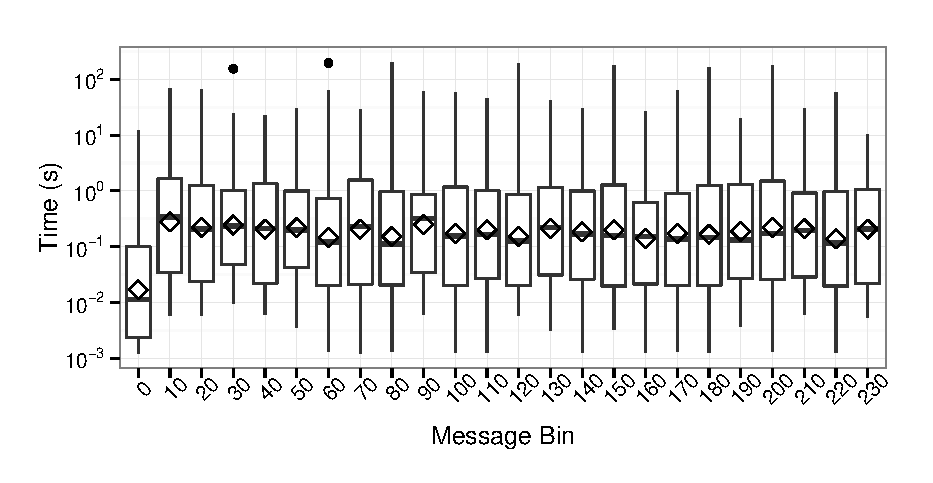
\epsfig{file=figures/ndss13/tetrinet_boxplot_bar_alt_log_Time_Default-Coarse.eps, width=0.6\columnwidth}
} \\[-5pt]
\subfigure[][Hint, $\clusters = \coarseClusterCount$]{
\label{fig:tetrinet:time:hint_coarse}
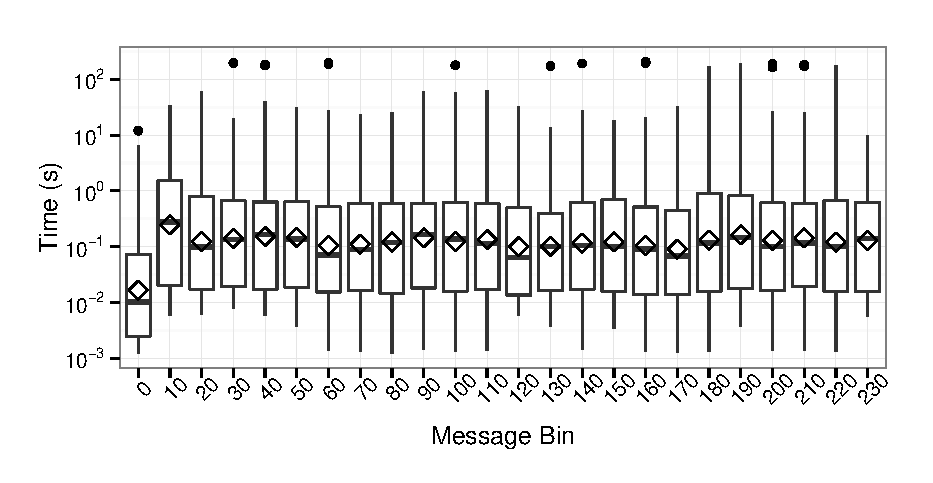
\epsfig{file=figures/ndss13/tetrinet_boxplot_bar_alt_log_Time_Hint-Coarse.eps, width=0.6\columnwidth}
} \\[-5pt]
\subfigure[][Default, $\clusters = \tetrinetFineClusterCount$]{
\label{fig:tetrinet:time:default_fine}
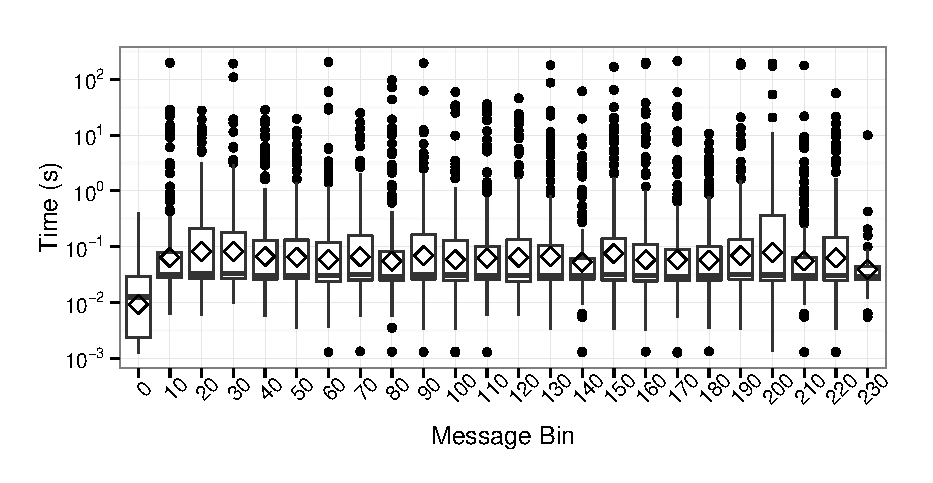
\epsfig{file=figures/ndss13/tetrinet_boxplot_bar_alt_log_Time_Default.eps, width=0.6\columnwidth}
} \\[-5pt]
\subfigure[][Hint, $\clusters = \tetrinetFineClusterCount$]{
\label{fig:tetrinet:time:hint_fine}
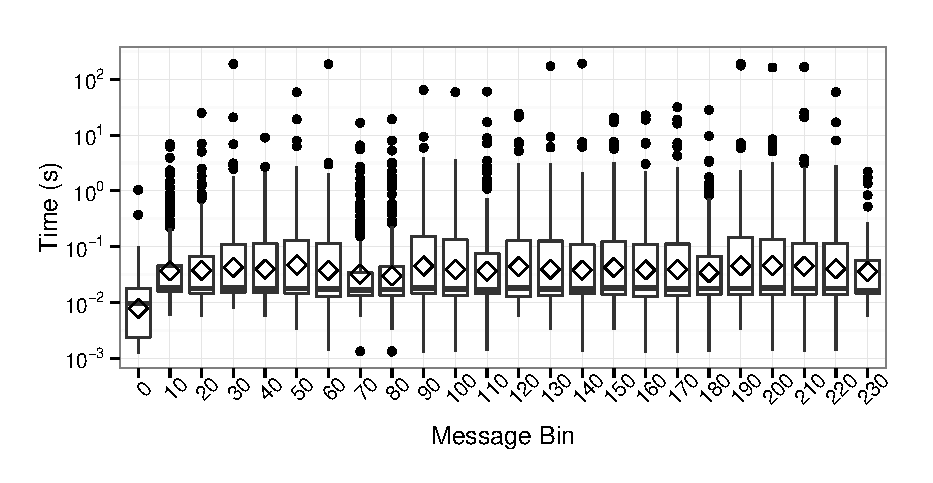
\epsfig{file=figures/ndss13/tetrinet_boxplot_bar_alt_log_Time_Hint.eps, width=0.6\columnwidth}
}\end{tabular}
\caption[\tetrinet verification costs.]{\tetrinet verification costs.
Cross-validation over \tetrinetTraces traces.  Boxplot at \xval shows
verification costs for messages \msg{\xval}, $\ldots$, \msg{\xval+9}
in each trace (after training on the other traces).  ``$\Diamond$''
shows the average.}
\label{fig:tetrinet:time}
\end{figure}


\begin{figure}[t]
\centering
\begin{tabular}{c}
\subfigure[][Default, $\clusters = \coarseClusterCount$]{
\label{fig:tetrinet:delay:default_coarse}
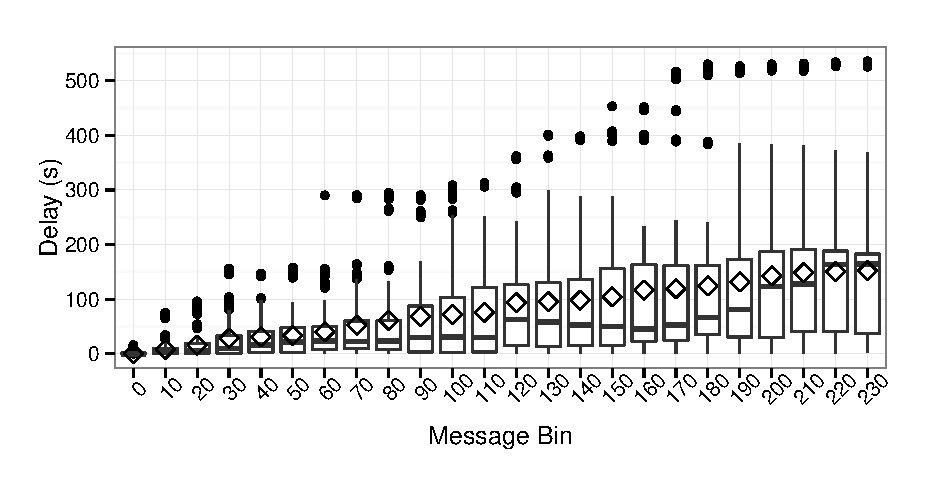
\epsfig{file=figures/ndss13/tetrinet_boxplot_bar_alt_Delay_Default-Coarse.eps, width=0.6\columnwidth}
} \\[-5pt]
\subfigure[][Hint, $\clusters = \coarseClusterCount$]{
\label{fig:tetrinet:delay:hint_coarse}
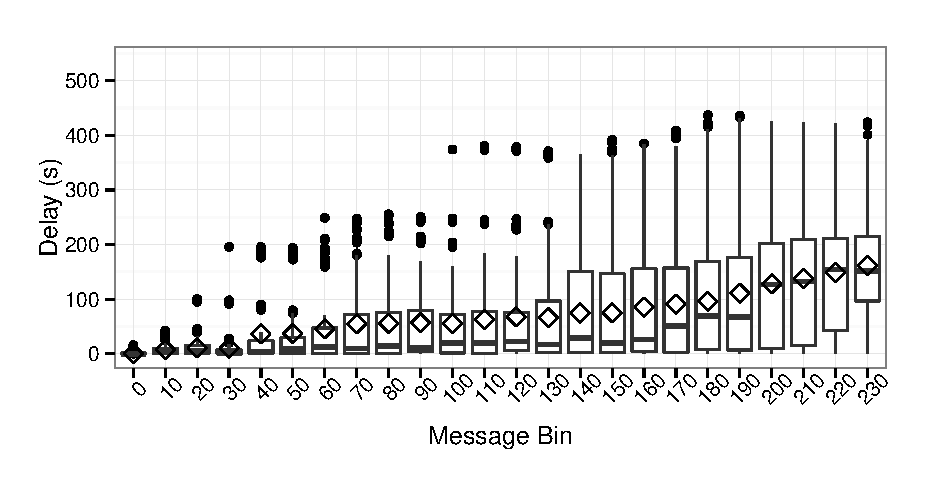
\epsfig{file=figures/ndss13/tetrinet_boxplot_bar_alt_Delay_Hint-Coarse.eps, width=0.6\columnwidth}
} \\[-5pt]
\subfigure[][Default, $\clusters = \tetrinetFineClusterCount$]{
\label{fig:tetrinet:delay:default_fine}
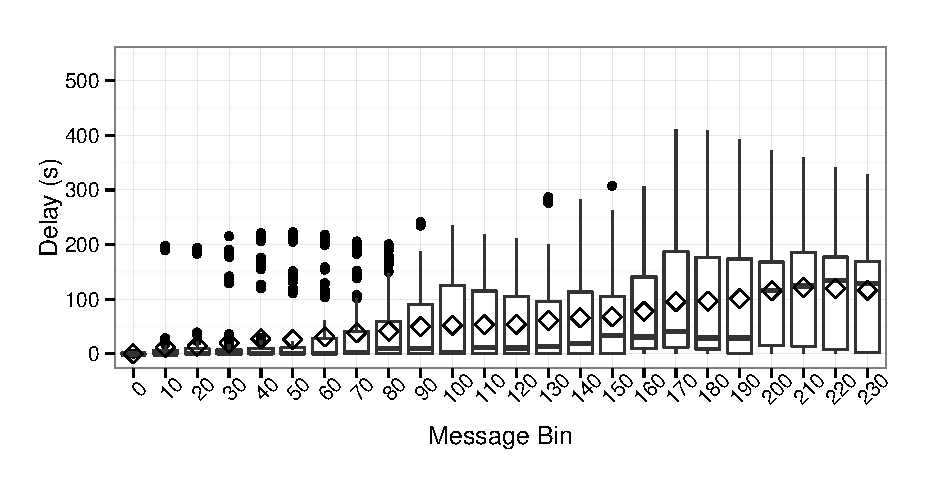
\epsfig{file=figures/ndss13/tetrinet_boxplot_bar_alt_Delay_Default.eps, width=0.6\columnwidth}
} \\[-5pt]
\subfigure[][Hint, $\clusters = \tetrinetFineClusterCount$]{
\label{fig:tetrinet:delay:hint_fine}
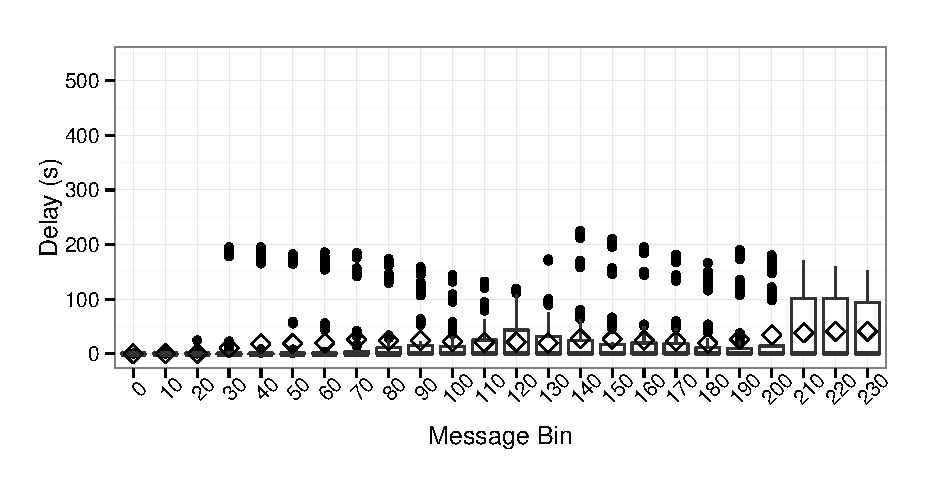
\epsfig{file=figures/ndss13/tetrinet_boxplot_bar_alt_Delay_Hint.eps, width=0.6\columnwidth}
}\end{tabular}
\caption[\tetrinet verification delays]{\tetrinet verification delays.
Cross-validation over \tetrinetTraces traces.  Boxplot at \xval shows
verification delays for messages \msg{\xval}, $\ldots$, \msg{\xval+9}
in each trace (after training on the other traces).  ``$\Diamond$''
shows the average.}
\label{fig:tetrinet:delay}
\end{figure}
\clearpage

To shed light on these issues, \figref{fig:tetrinet:delay} instead
plots the distributions of per-message verification \textit{delay}
between the arrival of message \msg{\msgNmbr} at the server (where a
server-to-client message ``arrives'' when it is sent) and the
discovery of an execution prefix \execPrefix{\msgNmbr} that is
consistent with \msg{0}, $\ldots$, \msg{\msgNmbr}.  Delay
(\figref{fig:tetrinet:delay}) differs from verification cost
(\figref{fig:tetrinet:time}) by representing the fact that
verification for \msg{\msgNmbr} cannot begin until after that for
\msg{\msgNmbr-1} completes.  So, for example, the rightmost boxplot
in each graph provides insight into how long after the completion of
the message trace (in real time) that it took for verification for the
whole trace to complete.

One item to note about these graphs is that for the hint configuration
with $\clusters = \tetrinetFineClusterCount$
(\figref{fig:tetrinet:delay:hint_fine}), the median of the rightmost
boxplot is virtually zero --- i.e., the most common case is that
verification kept pace with gameplay.  This can occur even if
verification falls behind at some point in the game, since
verification commonly ``catches up'' after falling behind. This is
illustrated, for example, in the generally downward slope of
consecutive outlier points in \figref{fig:tetrinet:delay:hint_fine}.
That said, the cumulative effect of verification delays in the other
configurations is more costly, e.g., causing verification to lag
behind gameplay by more than 100 seconds by the end of a
\tetrinetTraceLength-message trace in the median case in the default
configuration (\figref{fig:tetrinet:delay:default_fine}).

A breakdown of verification costs for \tetrinet is shown in
\figref{fig:time_summary}.  In our \tetrinet experiments,
more than 50\% of the verification cost is spent in \klee,
interpreting client instructions.  Therefore, optimizations that
interpret instructions only selectively (e.g.,~\cite{chipounov11:s2e})
may be a significant optimization for our tool.  The majority of the
remaining time is spent in insertions and deletions on \liveSet and in
computing edit distance, both to update the edit distance for each
path when a symbolic branch is reached and to compute distances
between messages.  A very small fraction of time in our \tetrinet
experiments is devoted to equivalent state detection
(\secref{sec:guided:verification:backtracking}) or in constraint solving.  In
\figref{fig:time_summary}, constraint solving includes not only the
time spent by \stp (the default solver used by \klee), but also
preprocessing techniques to make queries to \stp more efficient and a
canonicalization step (similar to Visser et
al.~\cite{visser12:canonicalization}) to improve the hit rate on
cached results for previous queries to \stp.  These optimizations
significantly reduce the overall constraint solving time.

\begin{figure}[H]
\centering
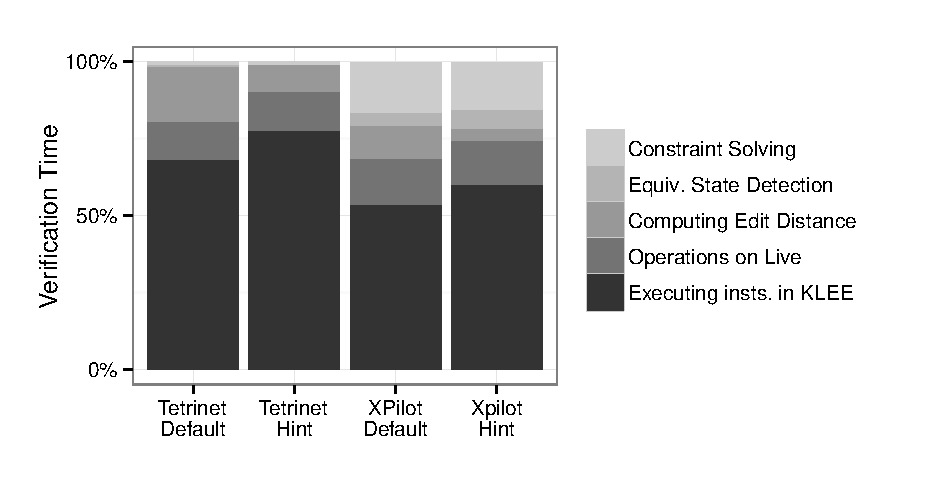
\epsfig{file=figures/ndss13/time_summary.eps, width=0.6\columnwidth}
\caption{Percentage of time spent in each component of the verifier.}
\label{fig:time_summary}
\end{figure}

\subsection{Case Study: \xpilot}
\xpilot poses a significant challenge for verification because its
pace is so fast.  The tests described here use an \xpilot
configuration that resulted in an average of \xpilotMsgsPerSec
messages per second.  The verification costs per message vary somewhat
less for \xpilot than they did for \tetrinet, as shown in
\figref{fig:xpilot:time}.  Recall that each boxplot in
\figref{fig:xpilot:time} represents $100 \times \xpilotTraces$ points,
versus only $10 \times \tetrinetTraces$ in \figref{fig:tetrinet:time}.
As such, though there are larger numbers of outliers in
\figref{fig:xpilot:time}, they constitute a smaller fraction of the
data points.

The median per-message verification cost of \xpilot when clustering is
fine-grained ($\clusters = \xpilotFineClusterCount$, which implied a
single execution fragment per cluster) is quite comparable to that in
\tetrinet, as can be seen by comparing
\figref{fig:xpilot:time:default_fine} and
\figref{fig:xpilot:time:hint_fine} to
\figref{fig:tetrinet:time:default_fine} and
\figref{fig:tetrinet:time:hint_fine}, respectively.  However, \xpilot
verification is considerably faster with coarse clustering, see
\figref{fig:xpilot:time:default_coarse} versus
\figref{fig:tetrinet:time:default_coarse} and
\figref{fig:xpilot:time:hint_coarse} versus
\figref{fig:tetrinet:time:hint_coarse}.  Our definition of $\clusters
= \coarseClusterCount$ as ``coarse'' clustering was dictated by the
goal of limiting the bandwidth overhead to one byte per
client-to-server message in the hint configuration.  The better
performance of \xpilot verification for coarse clustering versus
\tetrinet is at least partly because $\clusters = 256$ is closer to
fine clustering ($\clusters = \xpilotFineClusterCount$) in the case of
\xpilot than it is for \tetrinet ($\clusters = \tetrinetFineClusterCount$).
In the hint configuration, $\clusters = \coarseClusterCount$ increases
bandwidth use by \xpilot client-to-server messages by
\xpilotCoarseBandwidthPerc, and $\clusters = \xpilotFineClusterCount$
(\logXpilotFineClusterCount bits, sent in two bytes) increases it by
\xpilotFineBandwidthPerc.

Though the median per-message verification cost of \xpilot is
generally as good or better than that for \tetrinet, the faster pace
of \xpilot makes it much more difficult for verification to keep pace
with the game.  This effect is shown in \figref{fig:xpilot:delay}.  As
shown in this figure, none of the configurations or clustering
granularities permitted verification to keep up with gameplay, and 
the best default configuration ($\clusters = \xpilotFineClusterCount$)
included one run that required $8$ minutes past the end of the trace to
complete its verification (see
\figref{fig:xpilot:delay:default_fine}).  Consequently, for an
application as fast-paced and as complex as
\xpilot, our algorithm does not eliminate the need to save
traces for post hoc analysis.

Nevertheless, we stress that our algorithm accomplishes --- even if
with some delay --- what is for the approach in \chref{ch:scv}
completely intractable.  That is, recall
that the approach in \chref{ch:scv} utilized a restricted version of \xpilot in which the
number of user inputs per event loop iteration was artificially
limited; we have removed that limitation here (see
\secref{sec:guided:eval:apps}).  With these restrictions removed, the
previous approach is inherently unbounded for verifying some
messages, since it seeks to eagerly find \textit{all} paths that could
explain that message, of which there could be infinitely many.  Our
approach, in contrast, succeeds in verifying all messages in these
logs in bounded time and with per-message cost averaging under
$100\msecs$ in all configurations (\figref{fig:xpilot:time}).

A fractional breakdown of verification costs for \xpilot are shown in
\figref{fig:time_summary}.  While a majority of the cost is still
contributed by interpreting client instructions in \klee, the majority
is smaller in the case of \xpilot than it was for \tetrinet.  For
\xpilot, equivalent state detection
(\secref{sec:guided:verification:backtracking}) plays a more prominent role
than it did for \tetrinet, in part due to \xpilot's more complex memory
structure.  Moreover, due to the substantially more complex
constraints generated by \xpilot, constraint solving plays a much more
prominent role than it did for \tetrinet.

\ignore{
, which is larger in \xpilot which has a more complex memory
structure. Not shown, is the less than 0.5\% of the overall time spent
in the SMT (Satisfiability Modulo Theory) solver; which in our case is
\stp, the default solver used by \klee. The time spent in the SMT
solver is quite low, due largely to the optimizations we preform on
the constraints, which include the canonicalization of variable names
(\secref{sec:guided:canonicalization}), again this optimization takes a
larger portion of the overall verification time in \xpilot.
}

\clearpage
\begin{figure}[t]
\centering
\begin{tabular}{c}
\subfigure[][Default, $\clusters = \coarseClusterCount$]{
\label{fig:xpilot:time:default_coarse}
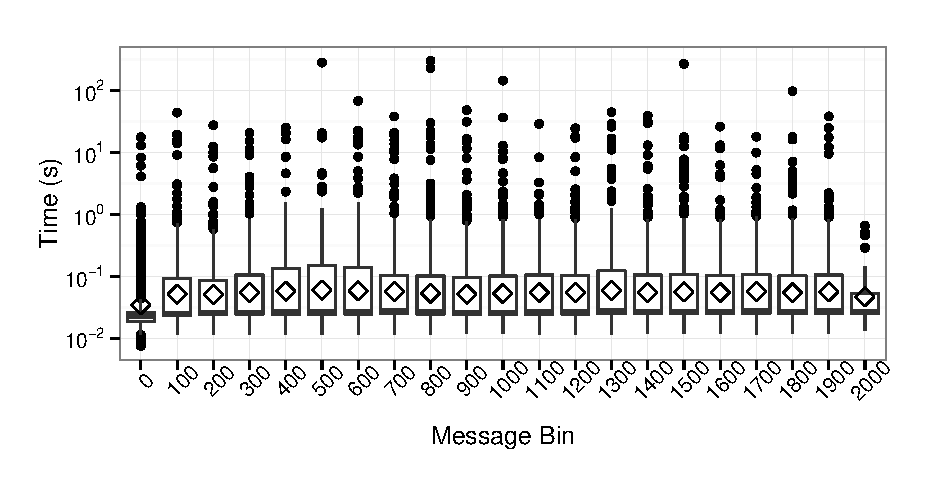
\epsfig{file=figures/ndss13/xpilot_boxplot_bar_alt_log_Time_Default-Coarse.eps, width=0.6\columnwidth}
} \\[-5pt]
\subfigure[][Hint, $\clusters = \coarseClusterCount$]{
\label{fig:xpilot:time:hint_coarse}
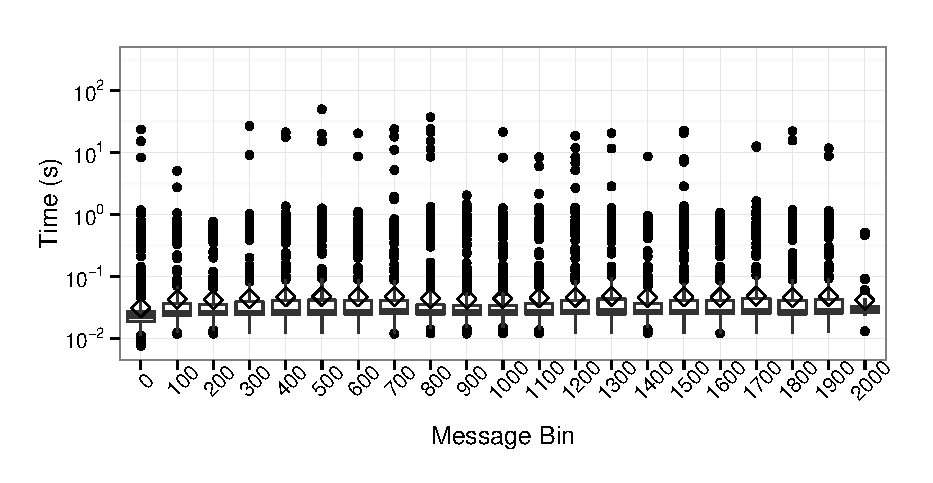
\epsfig{file=figures/ndss13/xpilot_boxplot_bar_alt_log_Time_Hint-Coarse.eps, width=0.6\columnwidth}
} \\[-5pt]
\subfigure[][Default, $\clusters = \xpilotFineClusterCount$]{
\label{fig:xpilot:time:default_fine}
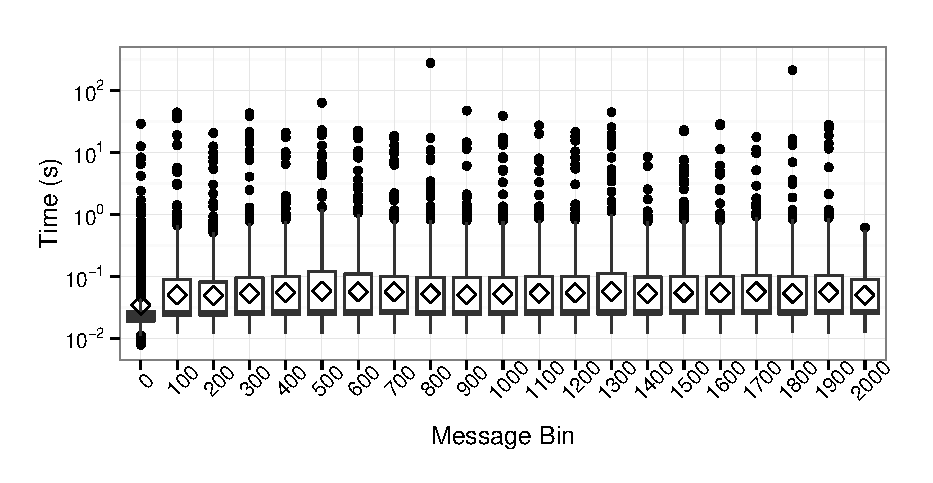
\epsfig{file=figures/ndss13/xpilot_boxplot_bar_alt_log_Time_Default.eps, width=0.6\columnwidth}
} \\[-5pt]
\subfigure[][Hint, $\clusters = \xpilotFineClusterCount$]{
\label{fig:xpilot:time:hint_fine}
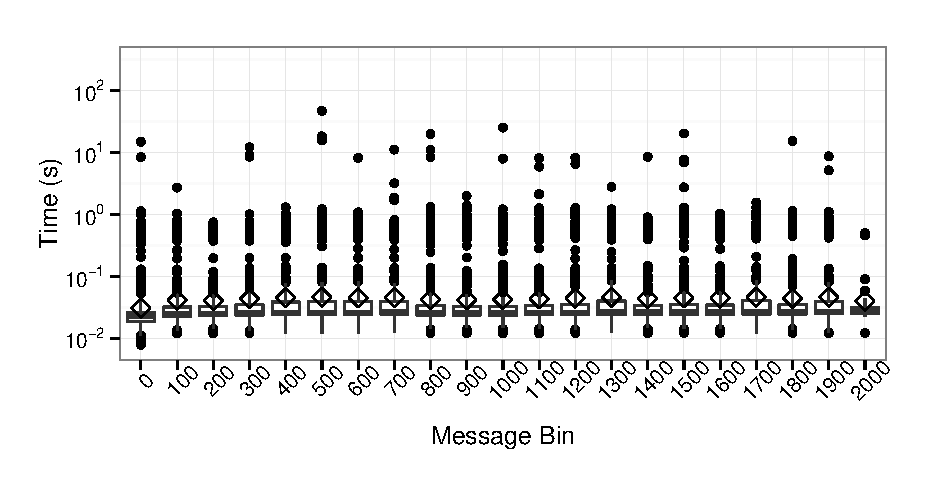
\epsfig{file=figures/ndss13/xpilot_boxplot_bar_alt_log_Time_Hint.eps, width=0.6\columnwidth}
}
\end{tabular}
\caption[\xpilot verification costs]{\xpilot verification costs.
Cross-validation over \xpilotTraces traces.  Boxplot at \xval shows
verification cost for messages \msg{\xval}, $\ldots$, \msg{\xval+99}
in each trace (after training on the other traces).  ``$\Diamond$''
shows the average.}
\label{fig:xpilot:time}
\end{figure}

\begin{figure}[t]
\centering
\begin{tabular}{c}
\subfigure[][Default, $\clusters = \coarseClusterCount$]{
\label{fig:xpilot:delay:default_coarse}
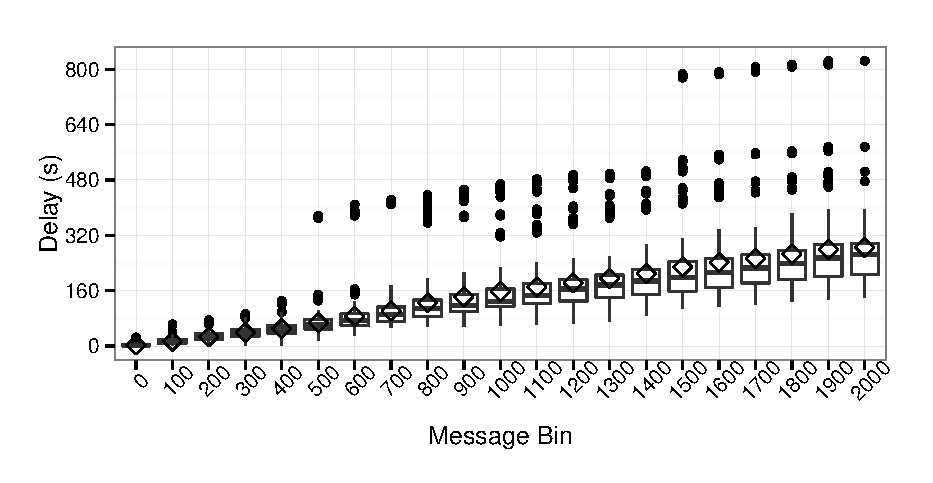
\epsfig{file=figures/ndss13/xpilot_boxplot_bar_alt_Delay_Default-Coarse.eps, width=0.6\columnwidth}
} \\[-5pt]
\subfigure[][Hint, $\clusters = \coarseClusterCount$]{
\label{fig:xpilot:delay:hint_coarse}
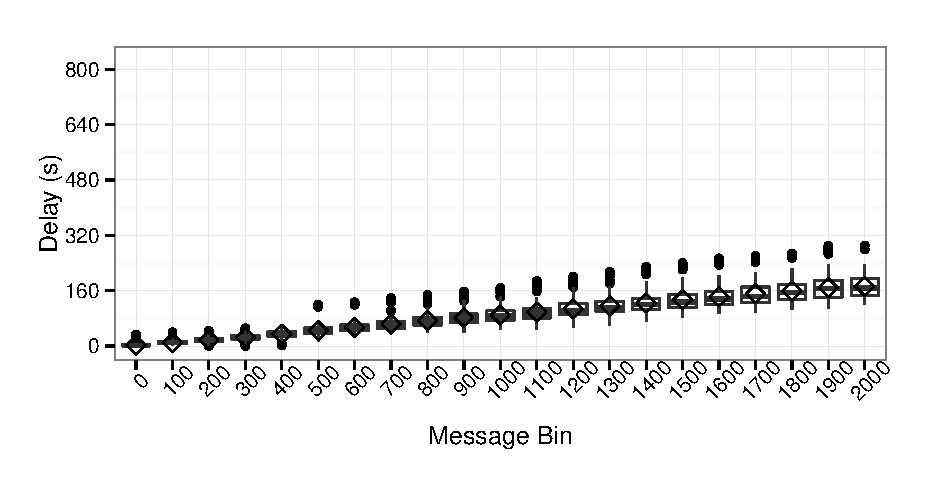
\epsfig{file=figures/ndss13/xpilot_boxplot_bar_alt_Delay_Hint-Coarse.eps, width=0.6\columnwidth}
} \\[-5pt]
\subfigure[][Default, $\clusters = \xpilotFineClusterCount$]{
\label{fig:xpilot:delay:default_fine}
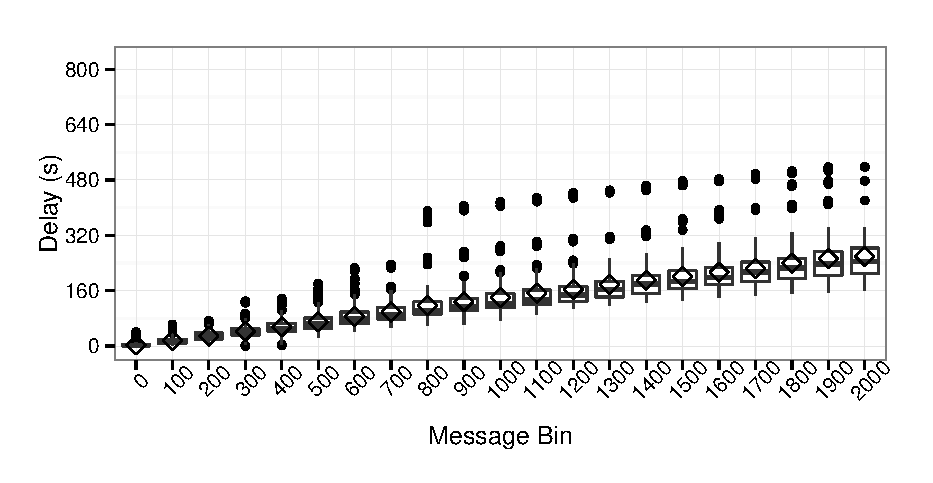
\epsfig{file=figures/ndss13/xpilot_boxplot_bar_alt_Delay_Default.eps, width=0.6\columnwidth}
} \\[-5pt]
\subfigure[][Hint, $\clusters = \xpilotFineClusterCount$]{
\label{fig:xpilot:delay:hint_fine}
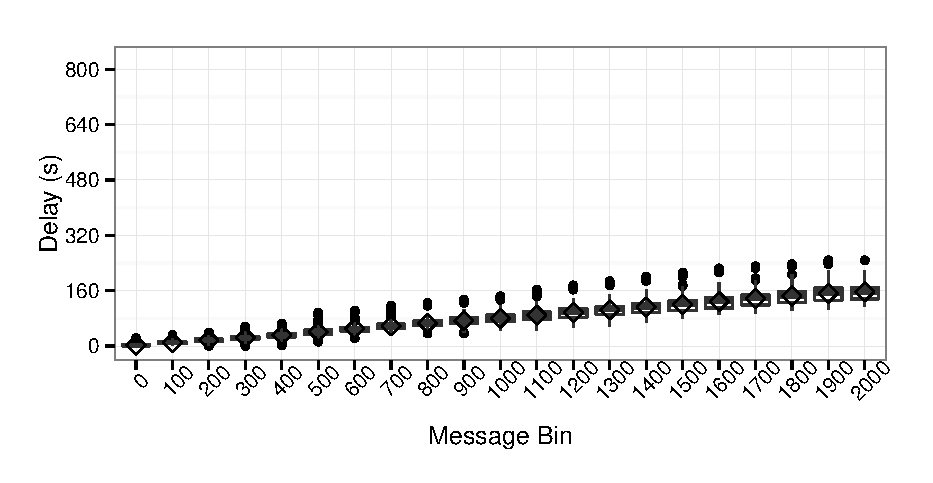
\epsfig{file=figures/ndss13/xpilot_boxplot_bar_alt_Delay_Hint.eps, width=0.6\columnwidth}
}
\end{tabular}
\caption[\xpilot verification delays]{\xpilot verification delays.
Cross-validation over \xpilotTraces traces.  Boxplot at \xval shows
verification delays for messages \msg{\xval}, $\ldots$, \msg{\xval+99}
in each trace (after training on the other traces).  ``$\Diamond$''
shows the average.}
\label{fig:xpilot:delay}
\end{figure}
\clearpage


\section{Summary}
\label{sec:guided:conclusion}

In this \paper we have presented a novel algorithm to enable a server
to verify that the behavior of a client in a client-server application
is consistent with the sanctioned client software.  The central
challenge that must be overcome in achieving this goal is that the
server does not know all of the inputs to the client (e.g., user
inputs) that induced its behavior, and in some domains
(see~\cite{mulligan03:guide}) the additional bandwidth utilized by
sending those inputs to the server is undesirable.  We therefore
developed a technique by which the verifier ``solves'' for whether
there exist user inputs that could explain the client behavior.  We
overcome the scaling challenges of this approach by leveraging execution history
to guide a search for paths through the client program that could
produce the messages received by the server.  This approach enables us to
achieve dramatic cost savings in the common case of a legitimate
client, and by allowing minimal additional bandwidth use, we can
improve performance even further.  In the best configuration of our
algorithm, verification of legitimate \tetrinet gameplay often keeps
pace with the game itself.  In other cases,
verification efficiency is adequate to practically handle client
applications that previous work was forced to restrict to make its
analysis tractable.  We believe that the manner in which we leverage
execution history can be useful in other applications of symbolic
execution, as well.



